\documentclass{article}
\usepackage[english]{babel}
\usepackage[utf8]{inputenc}
\usepackage[table]{xcolor}
\usepackage{graphicx}
\usepackage{float}
\usepackage{longtable}
\usepackage{rotating}
\usepackage{adjustbox}
\usepackage{booktabs}
\usepackage{caption}

\setlength{\parskip}{1em}


\usepackage{listings}


\usepackage{hyperref}
\hypersetup{
	colorlinks,
	citecolor=black,
	filecolor=black,
	linkcolor=black,
	urlcolor=black
}

\begin{document}

\begin{titlepage}
      \centering
      \begin{figure}
            \begin{center}
                  
\includegraphics[width=0.6\textwidth]{images/logo_polimi.png}
            \end{center}
      \end{figure}
      \vfill
      {\scshape\LARGE Software Engineering 2 Project\\Academic Year 2021 - 2022 \par}
      \vspace{0.8cm}
      {\scshape\LARGE DREAM}
      \vfill
      \newcommand{\HRule}{\rule{\linewidth}{0.3mm}}
      \centering
      \HRule \\[0.4cm]
      \huge  Design Document\\% Title of your document
      \HRule \\
      \vspace{1cm}
      {\Large Valeria \textsc{Detomas} \quad Sofia \textsc{Martellozzo} \par}
      \vfill
      {\large Professor\par
          Elisabetta \textsc{Di Nitto}}
      \vfill
      {\large \textbf{Version 1}\\ \today \par}
\end{titlepage}


\newpage
\renewcommand\contentsname{Contents}
\tableofcontents

\newpage

%-----------------------------------------------------------%
\section{Introduction}
\subsection{Purpose}
The purpose of this document is to thoroughly describe 
Data-dRiven PrEdictive FArMing in Telengana(DREAM).
It presents functional and non functional requirements of the system and its components.
Moreover it provides use cases and scenarios for the users involved.
\\This document is meant as a contractual basis for the customer and the developer.

\subsubsection{Goals}\label{section:1.1.1}
  \begin{table}[h]
        \rowcolors{1}{gray!25}{white}  
        \centering
  \begin{tabular}{|p{2cm}|p{9cm}|}
    \hline
    G1 & allow policy makers to retrieve information from farmers and to evaluate their performance\\
    \hline
    G2 & allow farmers to communicate with each other\\
    \hline
    G3 & allow farmers to insert data and advices on his production\\
    \hline
    G4 & allow farmers to send request of help to Policy Makers\\
    \hline
    G5 & allow farmers to retrieve information relevant for their activity\\
    \hline
    G6 & Policy Makers and farmers should be able to consult the map of the zone ( and the informations stored in it ) with different levels of visibility\\
    \hline
    G6A & Policy Makers and farmers should be able to see the position of the farms on the map\\
    \hline
    G6B & Policy Makers should be able to see both the information about the production and the evaluation of each farm\\
    \hline
    G6C & farmers should be able to see only the type of production of a farmer by the map\\
    \hline
  \end{tabular}
  \caption{Definition of goals}
\end{table}

\subsection{Scope}

The aim of the system is to acquire and combine data and information of farmers in Telengana. 
The system will provide support both to Telengana’s policy makers and to farmers 
thanks to new innovative technologies.\\
Through the system, policy makers are able 
to get a complete picture of the agriculture status in the whole state. In order 
to obtain this, Dream provides information that make policy makers able to give 
incentives to those farmers who are performing well. Moreover it allows them to 
keep track of those farmers who need help. \\
The farmers have access to a forum where they are able to communicate with other 
farmers. The aim of the forum is to share useful suggestions and to let farmers 
who struggle with something ask for help. \\
Therefore on the one side policy makers can have an entire perspective of the farms’ 
situation in the entire state and on the other side farmers can take advantage of the 
application and discuss with their colleagues.
\par 
Hence the application is used by the policy makers as a way to monitor farmers. 
Through the system they are able to search a farm and have access to its general information. 
Once a month they salso end each farmer an evaluation message where they specify if the farmer activity was
performed good or bad.\\
On the contrary farmers can ask for help or write advices. They are free to write messages and communicate with other farmers through a forum 
that is created especially for them.




\subsubsection{World Phenomena}
\begin{itemize}
    \item Farmer starts growing some type of crop
    \item Weather conditions influence production
    \item Telengana’s state collects data concerning meteorological forecasts
    \item Farmer uses water irrigation system
    \item Farmer is struggling with his harvest  
    
\end{itemize}

\subsubsection{Shared Phenomena}

\begin{itemize}
    \item Farmer access Dream
    \item Farmer sends a message in the forum
    \item The amount of water used by the farmer is registered on the application
    \item Farmer inserts data about his production in the system
    \item Farmer sends a help request to the policy maker
    \item A user visualizes the map that identifies the farms
    \item Policy maker evaluates farmers' performances
    \item A user checks notifications
    
\end{itemize}

\subsection{Glossary}
\subsubsection{Definitions}
\begin{itemize}
        \item \textbf{DBMS} is a software that works as an interface between the end user and the database. It manages the data, the database engine and the database schema.
        \item \textbf{HTTPS} is a protocol where encrypted HTTP data is transferred over a secure connection. It also guarantees the privacy and integrity of data.
        \item \textbf{API} is a programming code that helps communicate two different computer programmes.
\end{itemize}
\subsubsection{Acronyms}
\begin{itemize}
        \item \textbf{API}: Application Programming Interface
        \item \textbf{HTTPS}: Hypertext Transfer Protocol Secure
        \item \textbf{DBMS}: Data Base Management System
        \item \textbf{UML}: Unified Modelling Language
\end{itemize}
\subsubsection{Abbreviations}
\begin{itemize}
        \item \textbf{Gn} goal number n
        \item \textbf{Rn} requirement number n
        \item \textbf{DAn} domain assumption number n
        \item \textbf{UCn} use case number n
        \item \textbf{Sn} scenario number n
\end{itemize}

\subsection{Document Structure}
\begin{enumerate}
    \item \textbf{Introduction}\\
            This section offers an introduction and a brief overview of the system that is presented in the document. 
            It highlights the purpose of the system and the goals that are meant to be achieved with it. 
            At the end there is also a glossary that contains a list of definitions, acronyms and abbreviations.
            
    \item \textbf{Overall Description}\\
            This section starts with a product perspective that contains a description of the system's domain through a class diagram. 
            It includes also state diagrams which are used to give more details about the behavior of some objects in the model.
            The section contains also a clear description of the features offered by the system, 
            it identifies the actors involved and it describes their characteristics.
            At the end there are domain assumptions and general constraints.
            
    
    \item \textbf{Specif Requirements}\\
            This section enters into the details on how the system interacts with the external world. It describes 
            the interfaces that are required and offered through several visual mockups. 
            Moreover the section provides functional and nonfunctional requirements. Functional
            requirements are additionally described by use cases, sequence diagrams and scenarios.
            At the end the section focuses on nonfunctional requirements and various limitations that the system might face.

    \item \textbf{Formal Analysis using Alloy}\\
            This section provides the model described through Alloy language.
            
    \item \textbf{Effor Spent}\\
            This section has a record of the hours spent to complete this document.

\end{enumerate}




%-----------------------------------------------------------%
\newpage
\section{Architectural Design}
%---------------------%
\subsection{High-level components and their interaction}
In the following section it is provided a high level view of the architecture of the system, 
which is structured following the three logic layer:\\

\begin{figure}[H]
    \begin{center}
    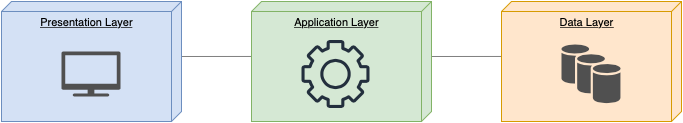
\includegraphics[width=1.2\textwidth]{images/System architecture.png}
    \caption{three layer architecture}
    \label{fig:system architecture}
    \end{center}
\end{figure}

\begin{itemize}
    \item \textbf{Presentation Layer (P)}: The presentation tier is the user interface and communication layer 
    of the application, where the end user interacts with the application. Its main purpose is to display 
    information to and collect information from the user. This top-level tier can run on a web browser, 
    as desktop application, or a graphical user interface (GUI), for example. \\ \\Web presentation tiers 
    are usually developed using HTML, CSS and JavaScript. Desktop applications can be written in a variety 
    of languages depending on the platform.
    \item \textbf{Business Logic or Application Layer(L)}: The application tier is the heart of the application. 
    In this tier, information collected in the presentation tier is processed - sometimes against other information in the data tier - 
    using business logic, a specific set of business rules. The application tier can also add, delete or modify data in the data tier.\\ \\
    The application tier is typically developed using Python, Java, Perl, PHP or Ruby, and communicates with the data tier using API calls. 
    \item \textbf{Data Layer (D)}: The data tier, sometimes called database tier, data access tier or back-end, is where the information 
    processed by the application is stored and managed. This can be a relational database management system such as PostgreSQL, MySQL, MariaDB, 
    Oracle, DB2, Informix or Microsoft SQL Server, or in a NoSQL Database server such as Cassandra, CouchDB or MongoDB. 
\end{itemize}

In this case the system is a distributed application that follows the client-server paradigm: it is a two-tier architecture, consisting of a presentation and a data tier. 
The business logic lives in the data tier only.
In a two-tier application, all communication goes through the application tier. The presentation tier and the data tier cannot communicate directly with one another. 

Client and server are being allocated into different physical machines and their communication takes place via other components and interfaces, located in the middle of the structure and composed by hardware and software modules. 
The client is a Web Application, which is by definition a thin client, because of its total dependency from the server; so it only contains the presentation layer.

\begin{figure}[H]
    \begin{center}
    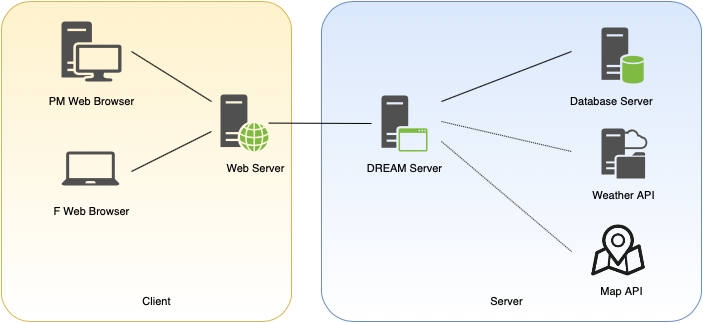
\includegraphics[width=1.2\textwidth]{images/System diagram.png}
    \caption{Dream system diagram.}
    \label{fig:system diagram}
    \end{center}
\end{figure}

\begin{itemize}
    \item \textbf{Server side:}
        \begin{itemize}
            \item \underline{ApplicationServer (DREAM Server)}: it is the central point of the system. Is a server with all the application logic, that communicates with the other servers. 
            \item \underline{Database Server}: this is the server where all the application data are stored.
            \item \underline{Weather API}: external API used to retrieve data about weather in the territory. This information will be used to fill each farm page.
            \item \underline{Map API}: external API used to retrieve data about the territory.
        \end{itemize}
    \item \textbf{Client side:}
        \begin{itemize}
            \item \underline{Policy Maker Web Browser}: browser used by the policy maker from their work desk to access to the system
            \item \underline{Farmer Web Browser}: browser used by the farmer to access to the system
        \end{itemize}
\end{itemize}


%---------------------%
\subsection{Component view}

In this section it is provided a description of the components and interfaces of the system, how they are organized internally and how they communicate with each other.

\subsubsection{High Level}

\begin{figure}[H]
    \begin{center}
    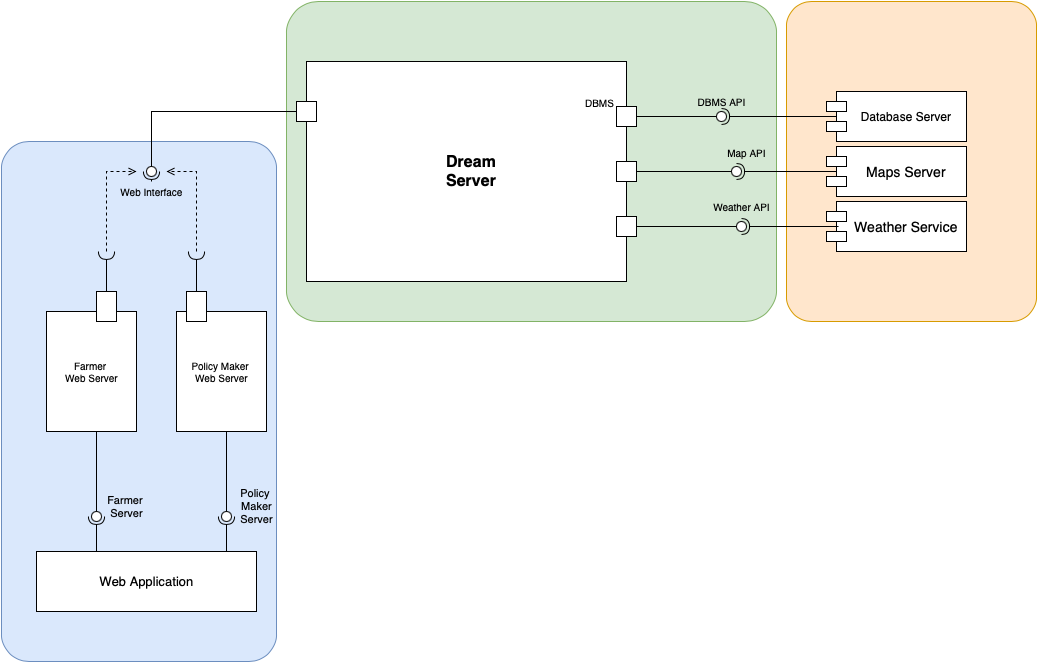
\includegraphics[width=1\textwidth]{images/Component3.png}
    \caption{Component view.}
    \label{fig:component view2}
    \end{center}
\end{figure}

\begin{itemize}
    \item \textbf{Dream Server}: this component contains the hole application logic of the system. The interfaces it provides allow the user, both farmer and policy maker, to comunicate with the server; them also allow the server to interact with external system that provide different kind of data.
    \item \textbf{Web Application}: it rapresents the web application reachable by any web browser. It is the first component that any user uses to connect with the system.
    \item \textbf{Farmer Web Server}: it provides the interface to a farmer to interact with the system. It has the minimum logic to make visible the content of the application provided by the server of the system. 
    \item \textbf{PolicyMaker Web Server}: the same as the one above but specific for the policy maker.
    \item \textbf{Database Server}: it provides the interfaces in all the processes that need to require or store information from the database of the system
    \item \textbf{Maps Server}: it provides the interfaces when the Dream server needs the maps data to make it visible and fill it with all the farms in the sistem, locating them by the position provided from their owner in the registration phase.
    \item \textbf{Weather Server}: it provides the interfaces to Dream server to retreive weather data of the territory.
\end{itemize}

\subsubsection{Server}
More specific and detailed on the server inner components.

\begin{figure}[H]
    \begin{center}
    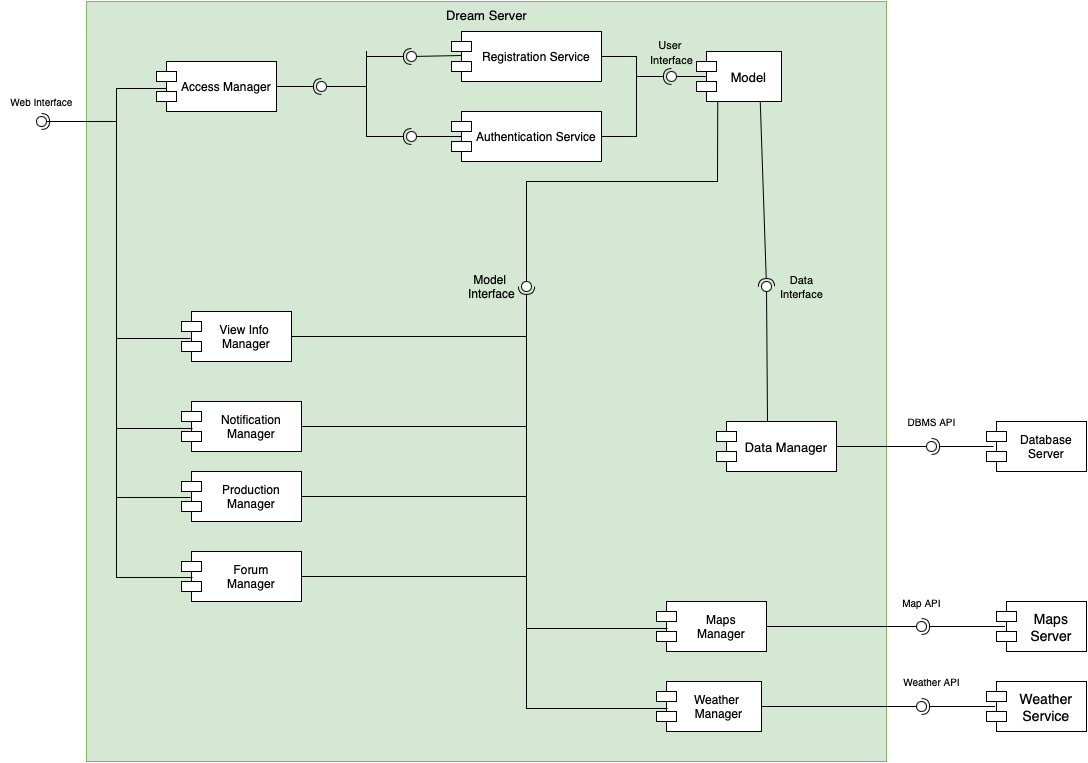
\includegraphics[width=1\textwidth]{images/ServerComponent3.png}
    \caption{Inner server component view2.}
    \label{fig:server component view2}
    \end{center}
\end{figure}

\begin{itemize}
    \item \textbf{Access Manager}: this component provide the Web interface to the user and make login and sign up opratation possible. It recognize the operation required and if it is permitted (sign up only for new farmers) comunicate with the right component that follow.
    \item \textbf{Registration Service}: if a request of a new registration occupr, it check the credential submitted by the new user and create the object that represent it, that will be stored in the Model; in fact it has an iterface to comunicate with the Model.
    \item \textbf{Authentication Service}: this component is called by the Access manager when an authentication request occur. In this case it collect the data about this specific user and verify if the credential submitted correspond. When them maches it let the user to access the system, otherwise generate an error signal.
    \item \textbf{ViewInfoManager}: this component is used by the system to collect the data from the Model request by the user. It operates when a farm's page has to be constructed with all the information visible in it.
    \item \textbf{Notification Manager}: this component has the ability to differ based on the notification it receives:
        \begin{itemize}
            \item advice: when a farmer submit this type of notification his only duty is the one to make possible the saving of it.
            \item help: when a farmer submit a request of help this component select randomly one policy maker (from the ones saved in the system) and send him the notification.
            \item solution: when a policy maker decides to respond to a request of help, he send this type of notification. This componenet forward it to the addressee.
            \item evaluation: when a policy maker evaluate a farm, this component takes care of sending it to the owner of the farm.
        \end{itemize}
    For all thee four type of notifications it attach the current day and time of the subbmission.
    This component also make possible to the user to visualize the list of all notifications received and, if asked, visualize in details the one selected.

    \item \textbf{Production Manager}: this component, by its connection to the model via \underline{Model interface}, povides all production data required for a specific farm. 
    \item \textbf{Forum Manager}: this component manage all the messages comunication between farmers via forum. It gets all the messages in it, saved as  List in the Model and comunicate to it the new ones, that has to mìbe saved (attaching to it the date and time).
    \item \textbf{Model}: this component have a main role in the system because it rapresents the data so all other components needs to interact with it, to ptovide the page and informations required.
    \item \textbf{Data Manager}: it manages all the process where data are needed by the system. It uses methods provided by the DBMS API to execute queries on the database and object-relational mapping to the Model.
    \item \textbf{Maps Manager}: this component is used to retreive map data, in order to provide a visualization of where each farmer registered in the system are located in the territory.
    \item \textbf{Weather Manager}: this component is used to retreive weather data specific in the position of the farms. It map to the Model the information from a relational to an object construct as a structure where the key is the farm position and in the value another structure to linked each day the weather and temperature.
\end{itemize}

%---------------------%
\subsection{Deployment view}
The deplyment diagram in figure \ref{fig:deployment} shows the allocation of the software components in the physical tiers of the system. 
The system is organized into a three-tier application. This type of architecture can be 
beneficial because each tier can be developed in parallel and maintained as single modules on separate platforms.


\begin{itemize}
    \item \textbf{Presentation Tier}: it is the user interface of the application, where the user interacts with the application. 
    In this case it can only be a computer with a web browser running on an operating system (for example MacOS).
    It is composed by the web app an the web server. The web server is responsible for the communication between application server 
    and the client.

    \item \textbf{Application Tier}: it is the logic tier of the application. Where all the information 
    collected in the previous tier are processed using business logic. This tier is also 
    responsible for the communication with the data tier through the DBMS gateway.
    The most important thing is that all communication of the system goes through this tier.

    \item \textbf{Data Tier}: it is a database server for managing read and write access to the database. 
    Therefore all the information processed by the application tier are stored and managed here.
    Data tier is also independent of the two previous tiers. 
\end{itemize}

\begin{figure}[H]
    \begin{center}
    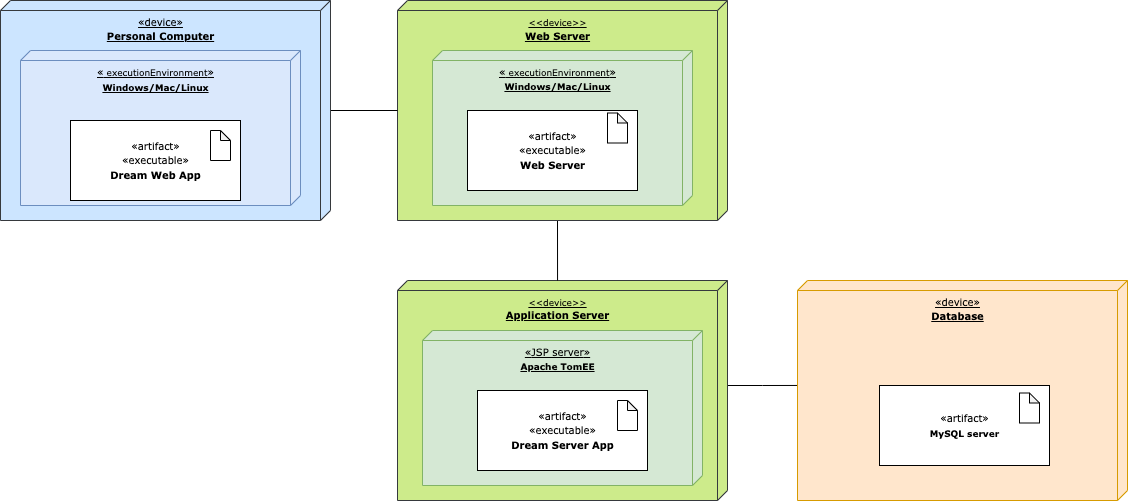
\includegraphics[width=0.7\textwidth]{images/Deployment diagram.png}
    \caption{\emph{Deployment} diagram}
    \label{fig:deployment}
    \end{center}
\end{figure}
%---------------------%
\subsection{Runtime view}

In this section the focus is on the specific (dynamic) interaction between the components of the system; in other world the behaviour of the system at runtime.
The functionality offered by the component are the same as the ones in the RASD, but this time the focus is on how the internal components provides it.
(MAKE SURE THAT THE OPERATION AND COMPONENT ARE ALL DEFINED IN THE COMPONENT DIAG/VIEW, in particular the interfaces that receives the msg)

\begin{enumerate}
    \item \textbf{farmer registration}\\
    In this sequence diagram is shown the sign up operation by a new farmer. After the user fill the form provided by the web application with: name, surmane, farm's name, position, email and password. The Dream server stores all this information as a Farmer object in the Model, and also saves them in the database. At the end of the process redirects the user to the login page, only if some error occurred the data are not saved and the user is asked to repeat the operation.
    \begin{figure}[H]
        \begin{center}
        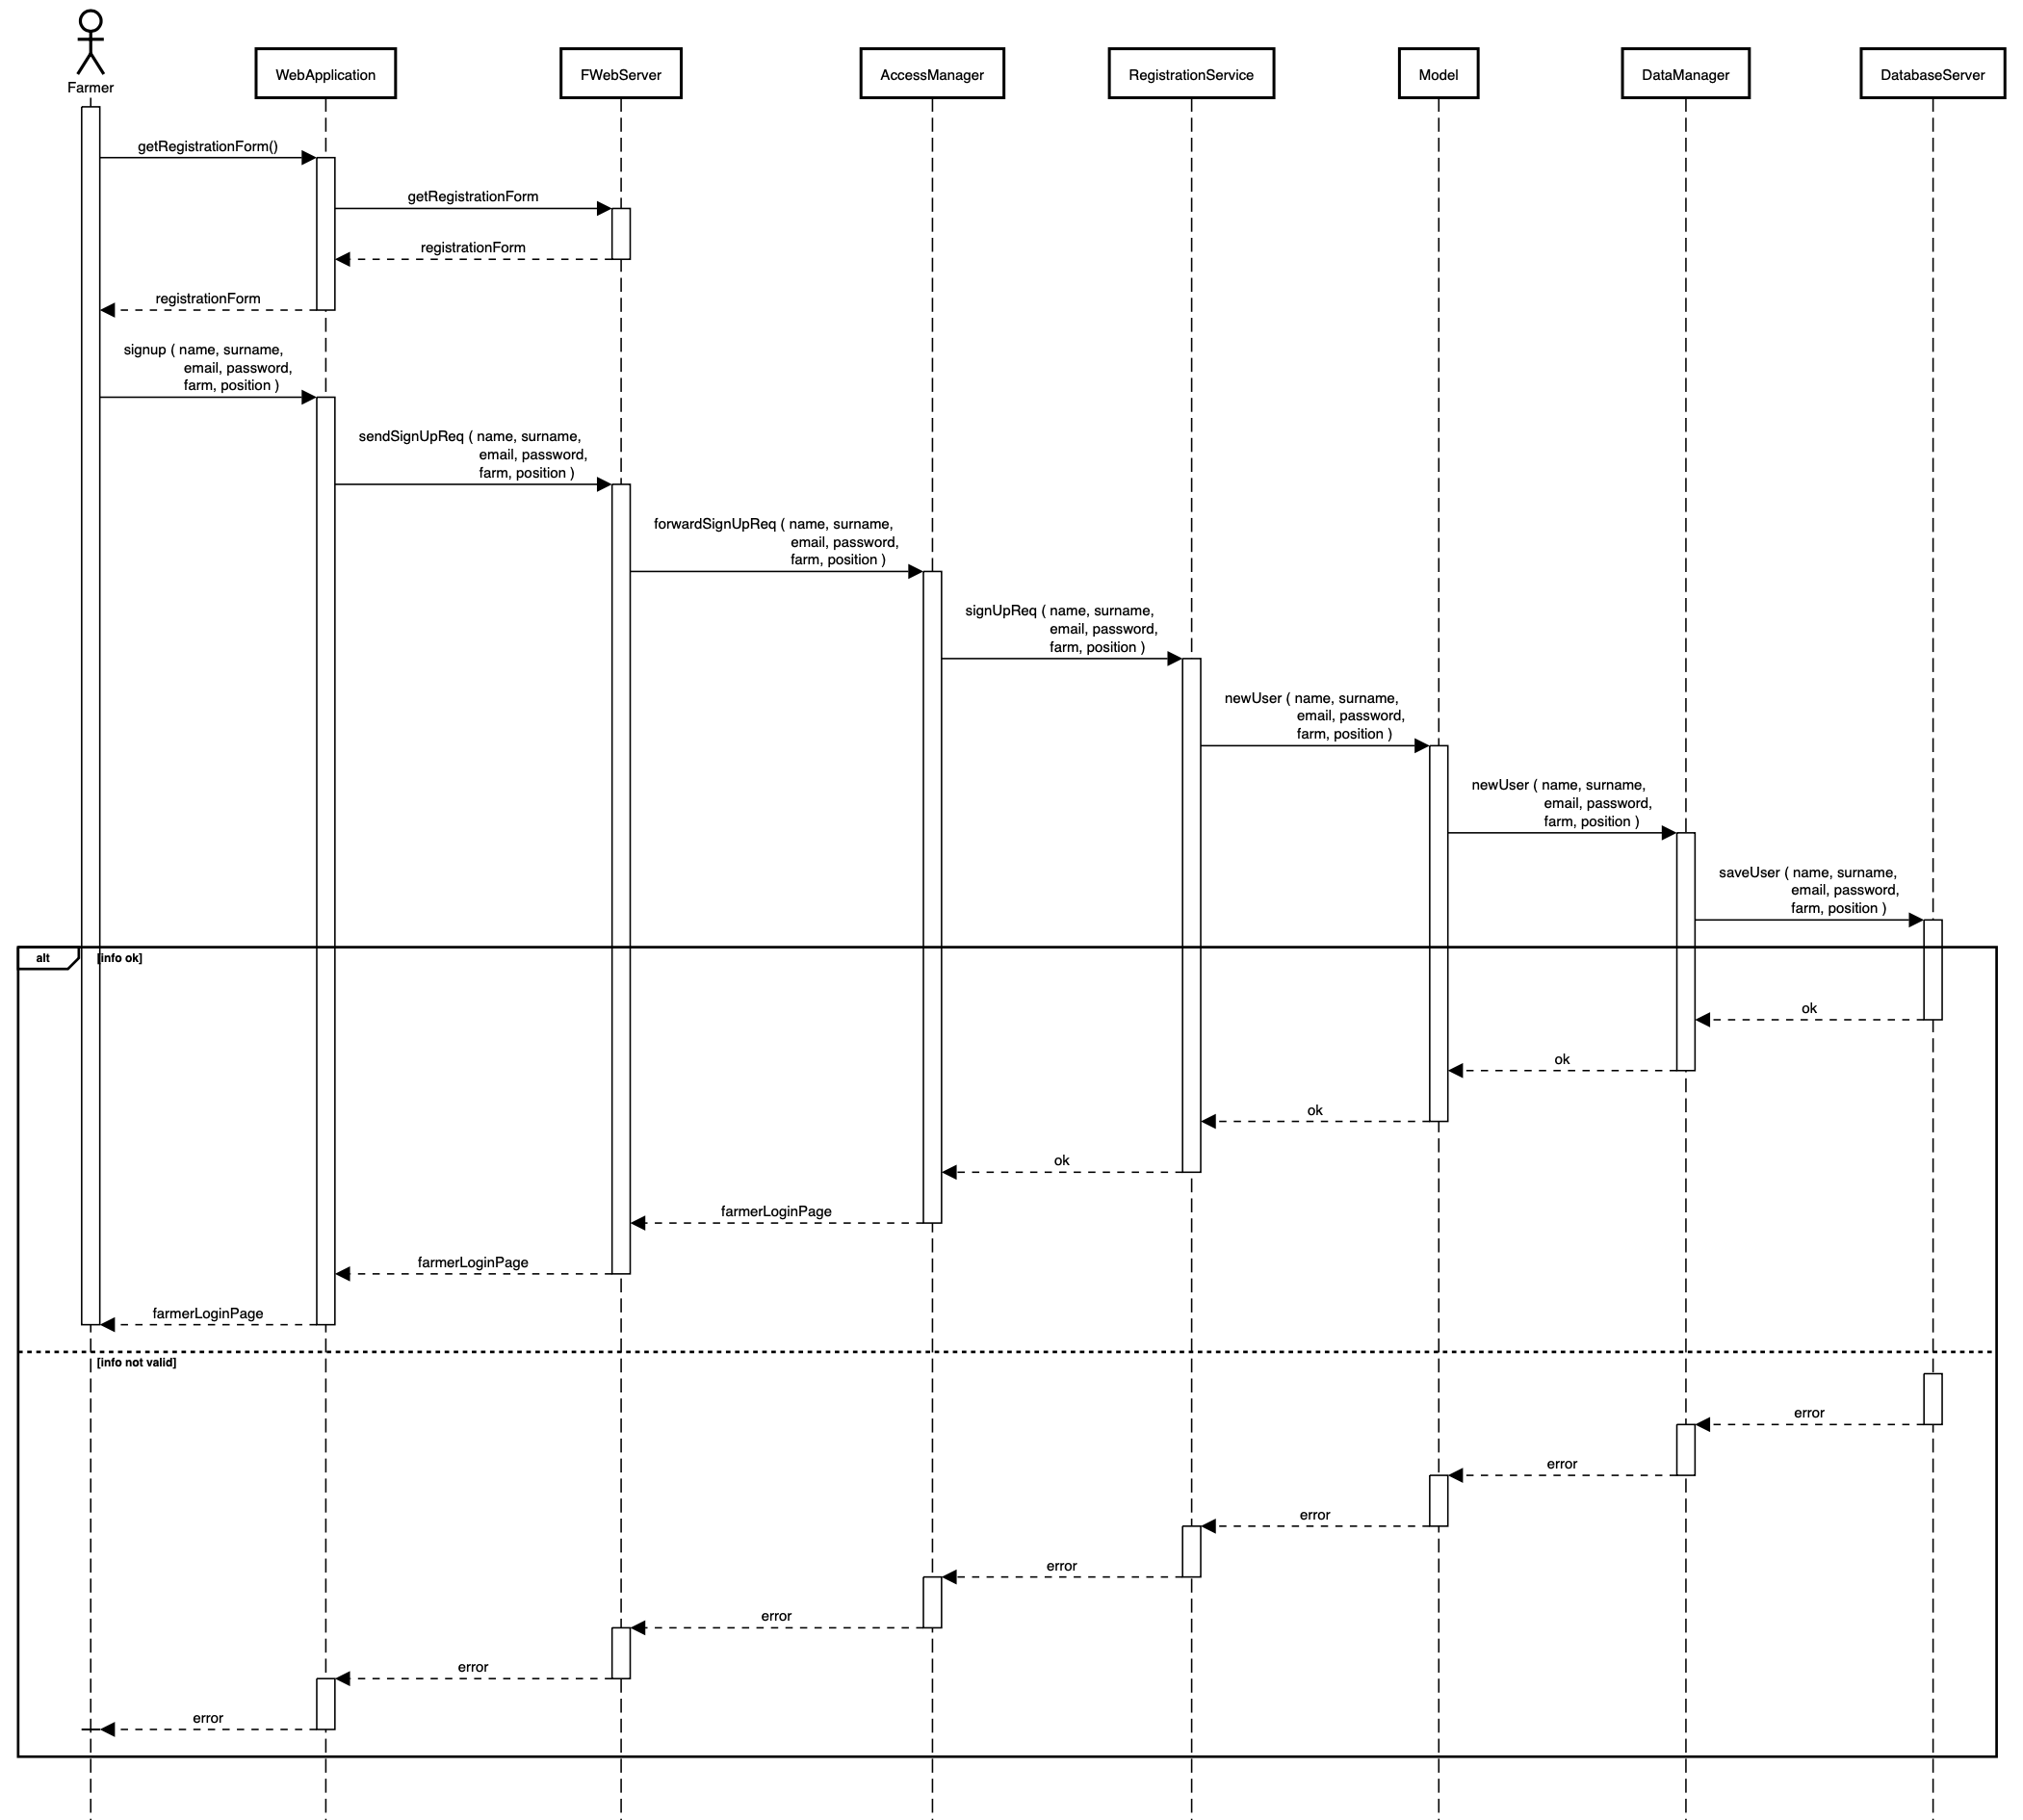
\includegraphics[width=0.7\textwidth]{sequence/signup.png}
        \caption{\emph{SignUp} sequence diagram}
        \label{fig:sequence1}
        \end{center}
    \end{figure}
    \item \textbf{login}\\
    In this sequence diagram the process of user login is shown, at first for the farmer and then for the policy maker. For both are almost the same, except that the farmers needs to provide email and password as access credentials and the policy maker a code and password. Another difference is in the server that forward the request to login to the Dream server component. If the credentials are wrong or missing the system gave an error message, if not the home page of the user is returned.
    \begin{figure}[H]
        \begin{center}
        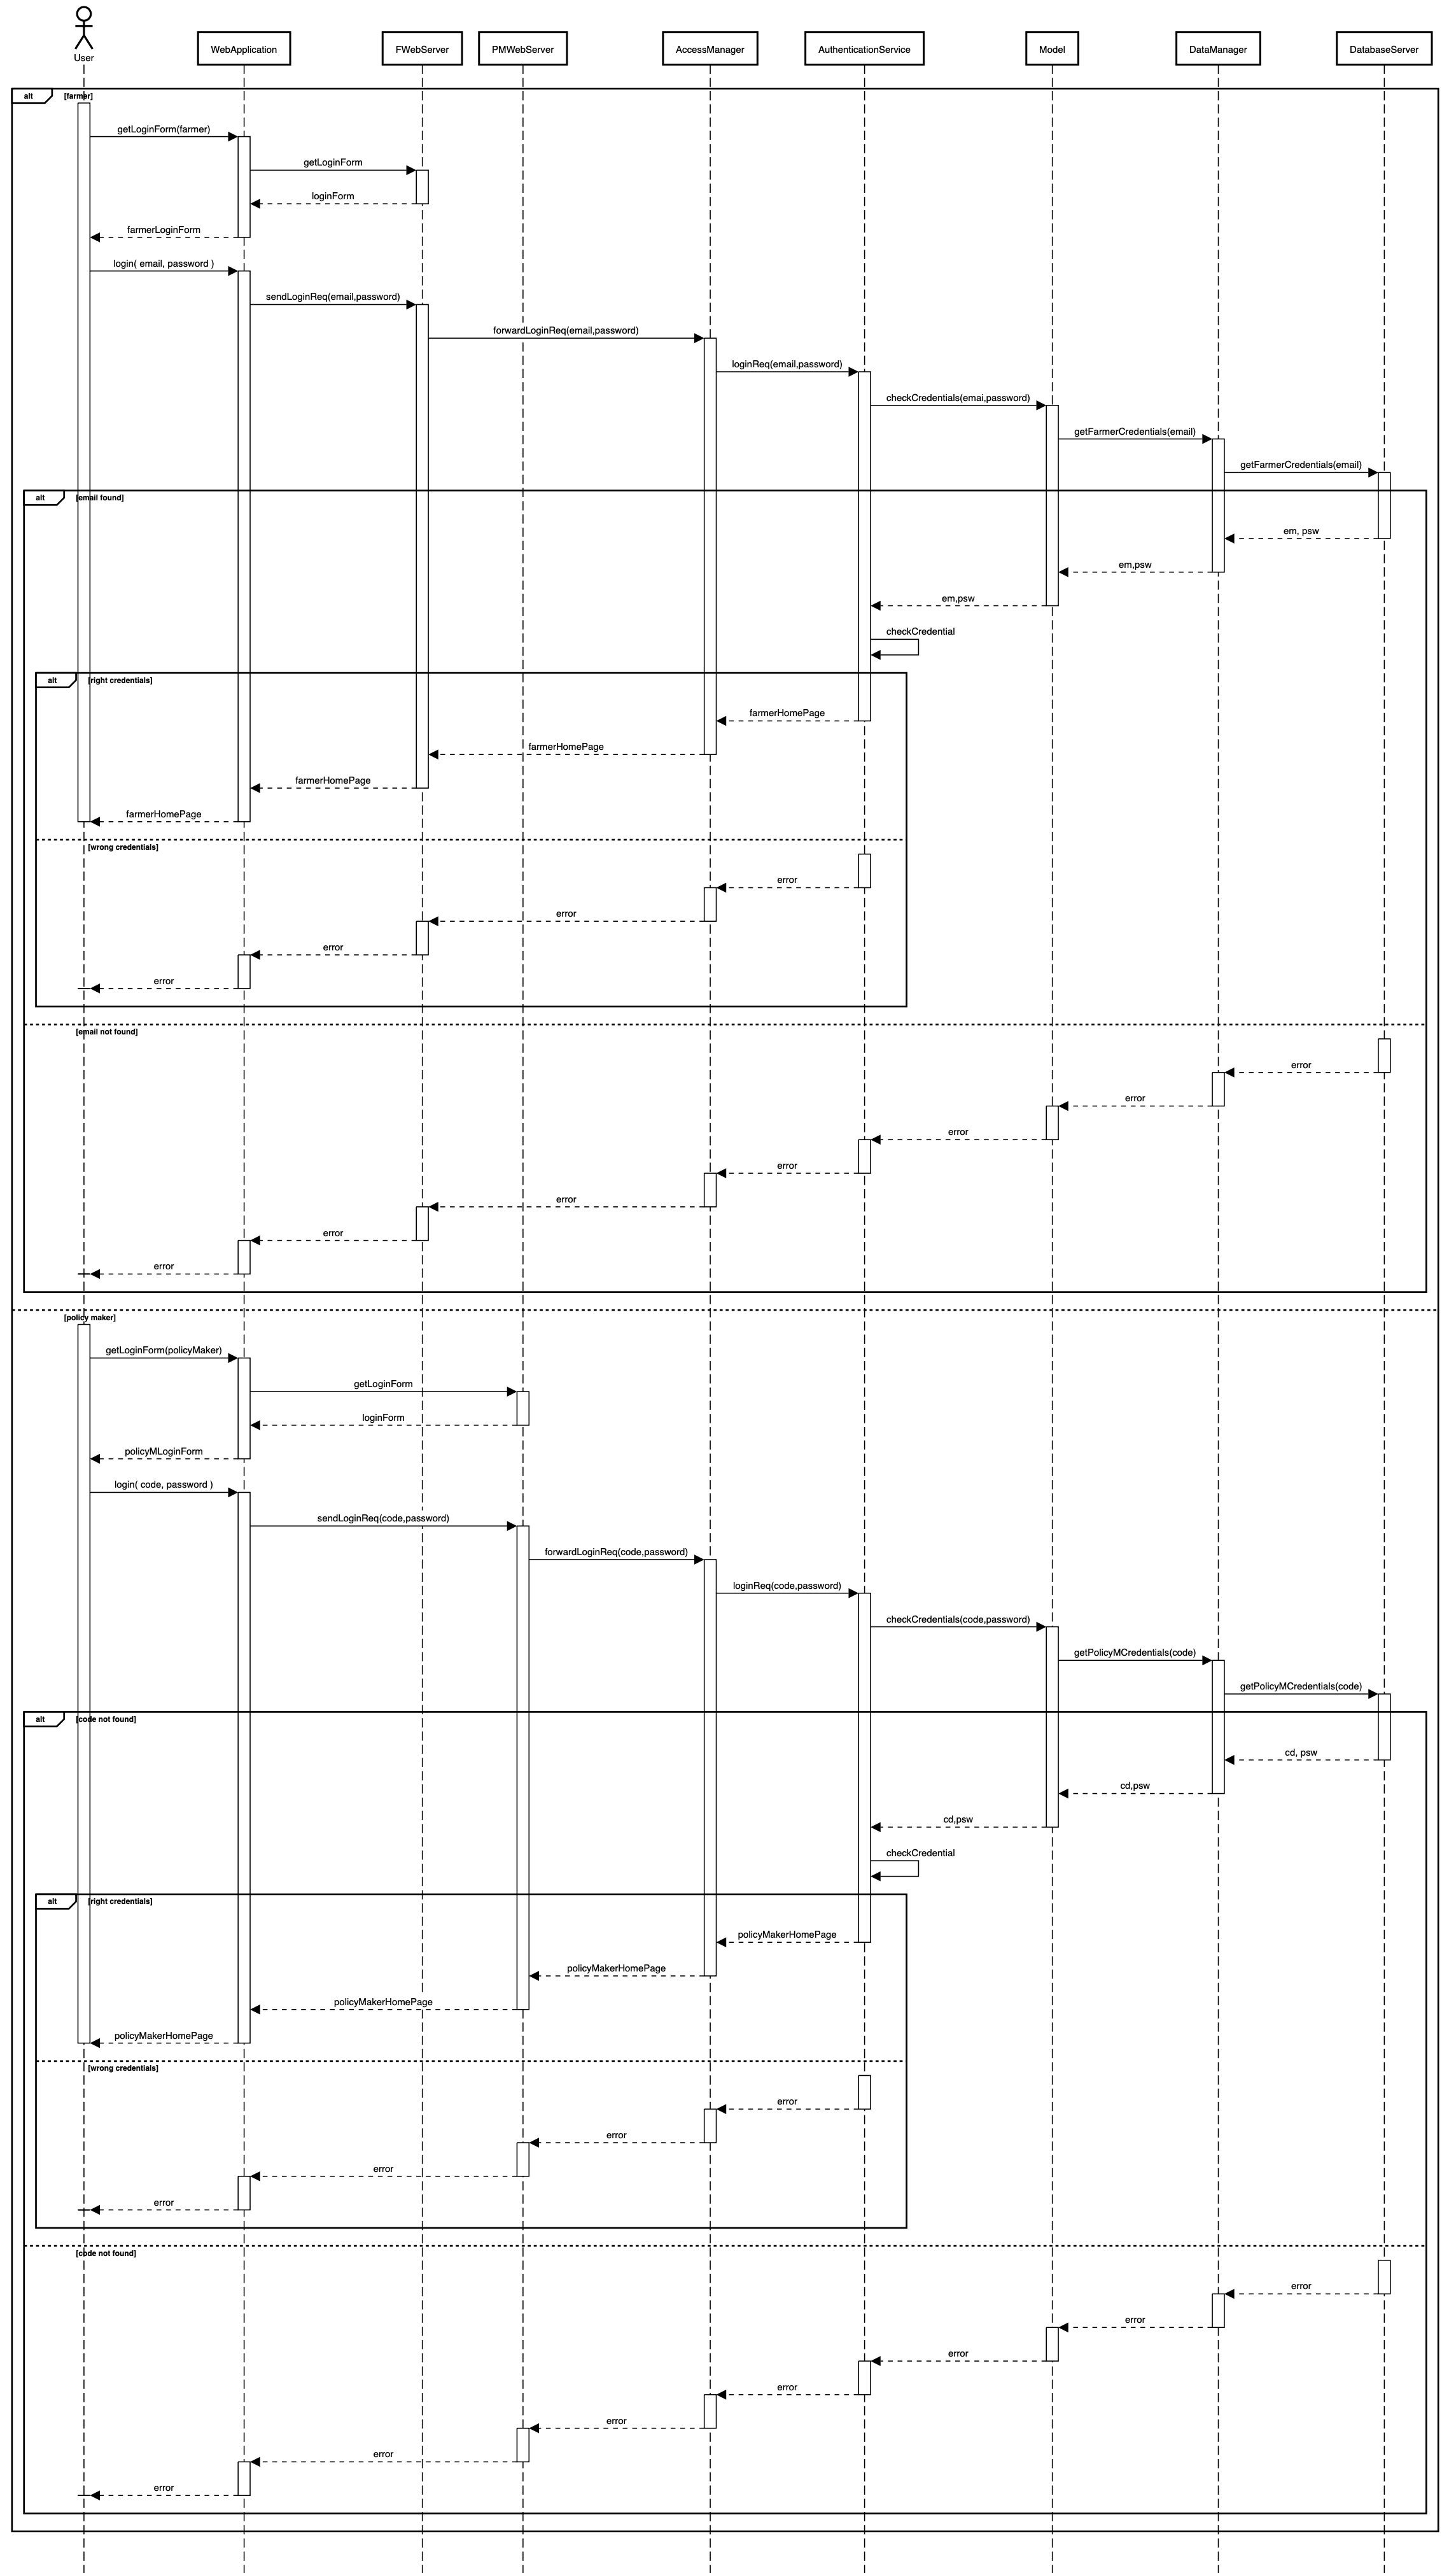
\includegraphics[width=0.7\textwidth]{sequence/login.png}
        \caption{\emph{Login} sequence diagram}
        \label{fig:sequence2}
        \end{center}
    \end{figure}
    \item \textbf{farmer read and write on forum}\\
    In this sequence is shown how the system provides the forum with all the messages yet sended after the request of a farmer and a form where he can write a message and a button to send it. As shown, due to the Forum Manager, when a message is send it is saved whit the references of the sender and the date and time. These addictonal information are used to sort the messages by the timestamp and specify the sender name near the message itself.
    \begin{figure}[H]
        \begin{center}
        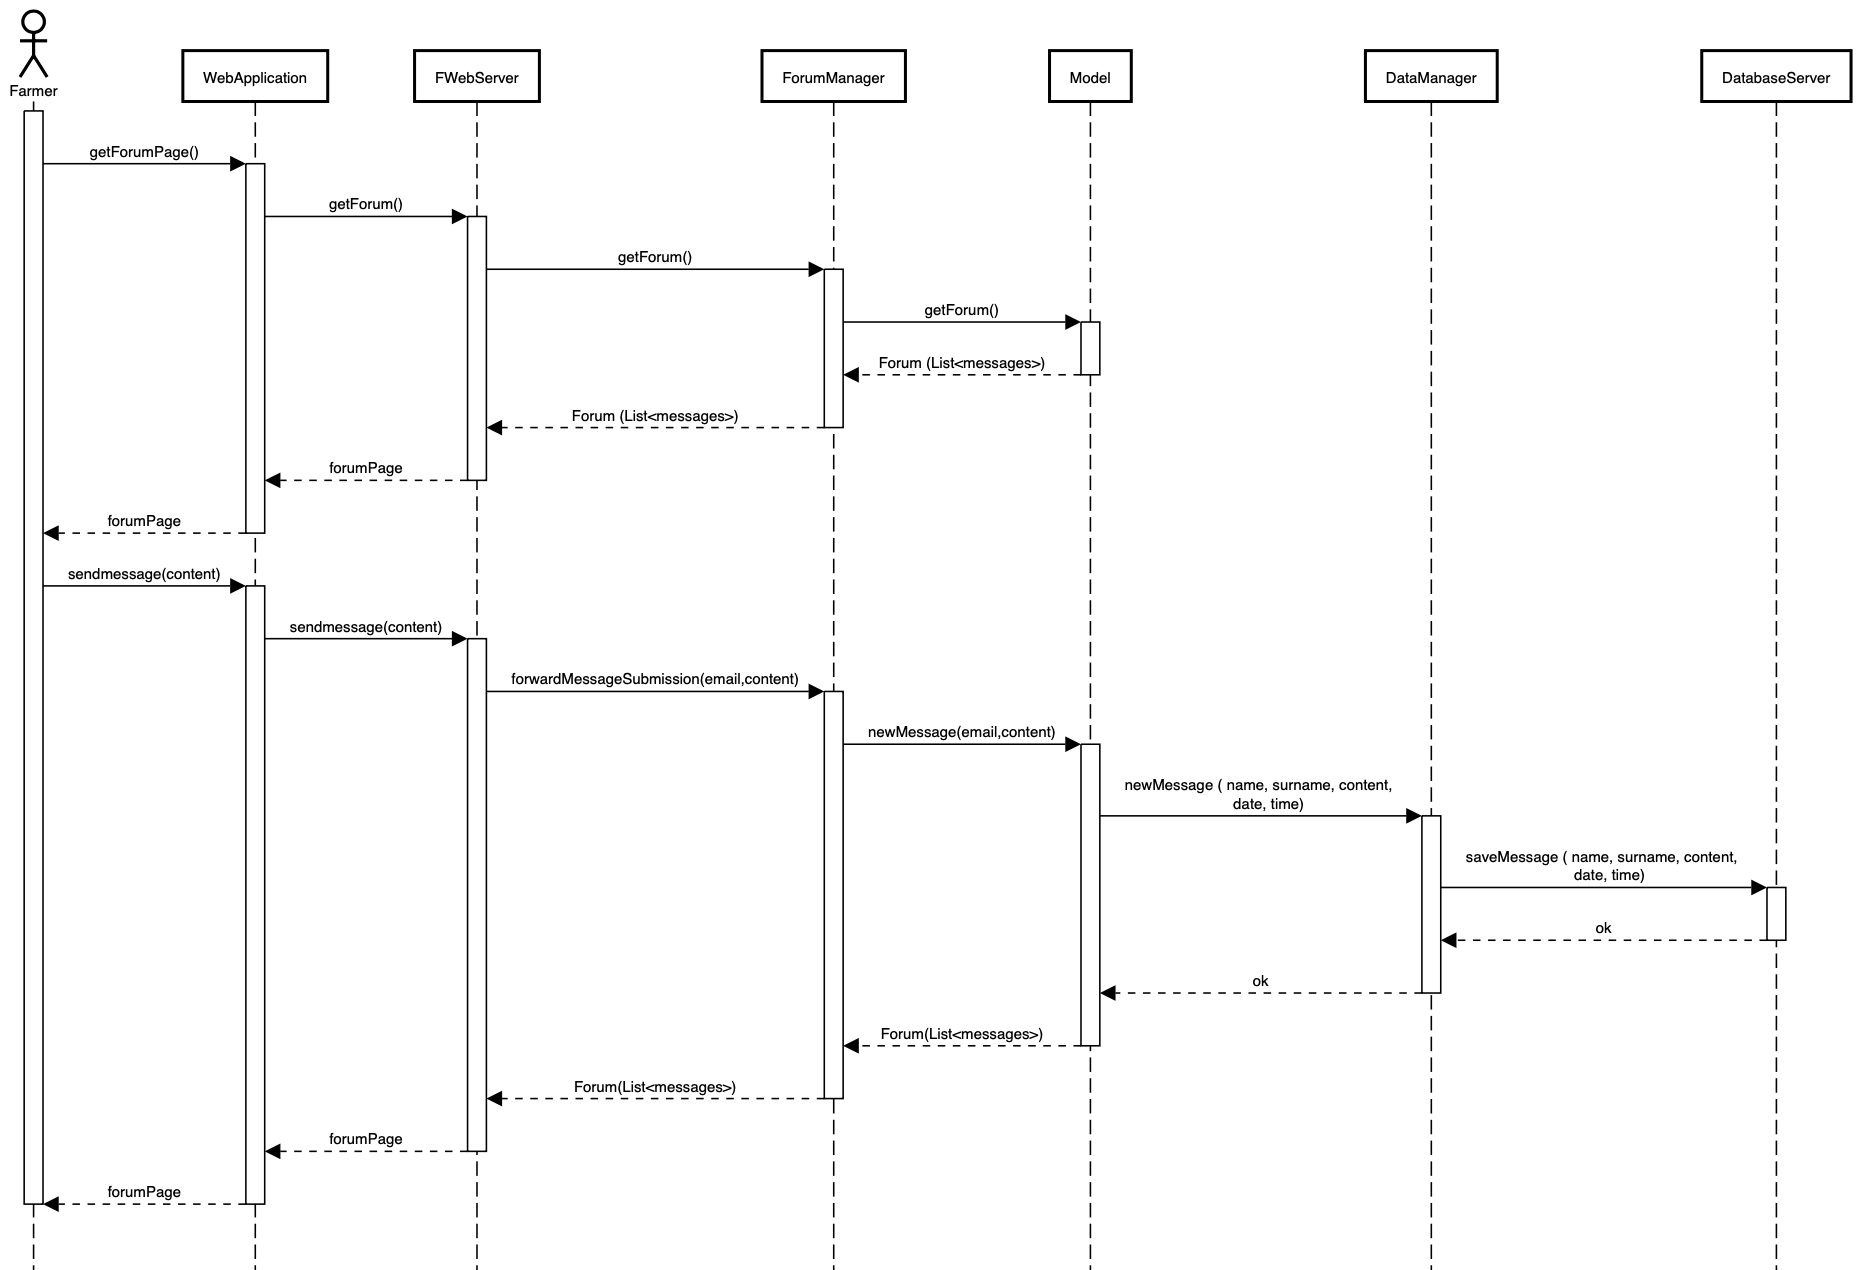
\includegraphics[width=0.7\textwidth]{sequence/forum.png}
        \caption{\emph{Save message} sequence diagram}
        \label{fig:sequence3}
        \end{center}
    \end{figure}
    \item \textbf{farmer submit production data}\\
    Here is shown how a farmer can submit new information about his production. The Web Application provides him a form to fill with the type of production, the quantity collected and the date on which he collected it. The Server, or better its Production Manager component, build this information as an object collected in the Model and saved then in the database.
    \begin{figure}[H]
        \begin{center}
        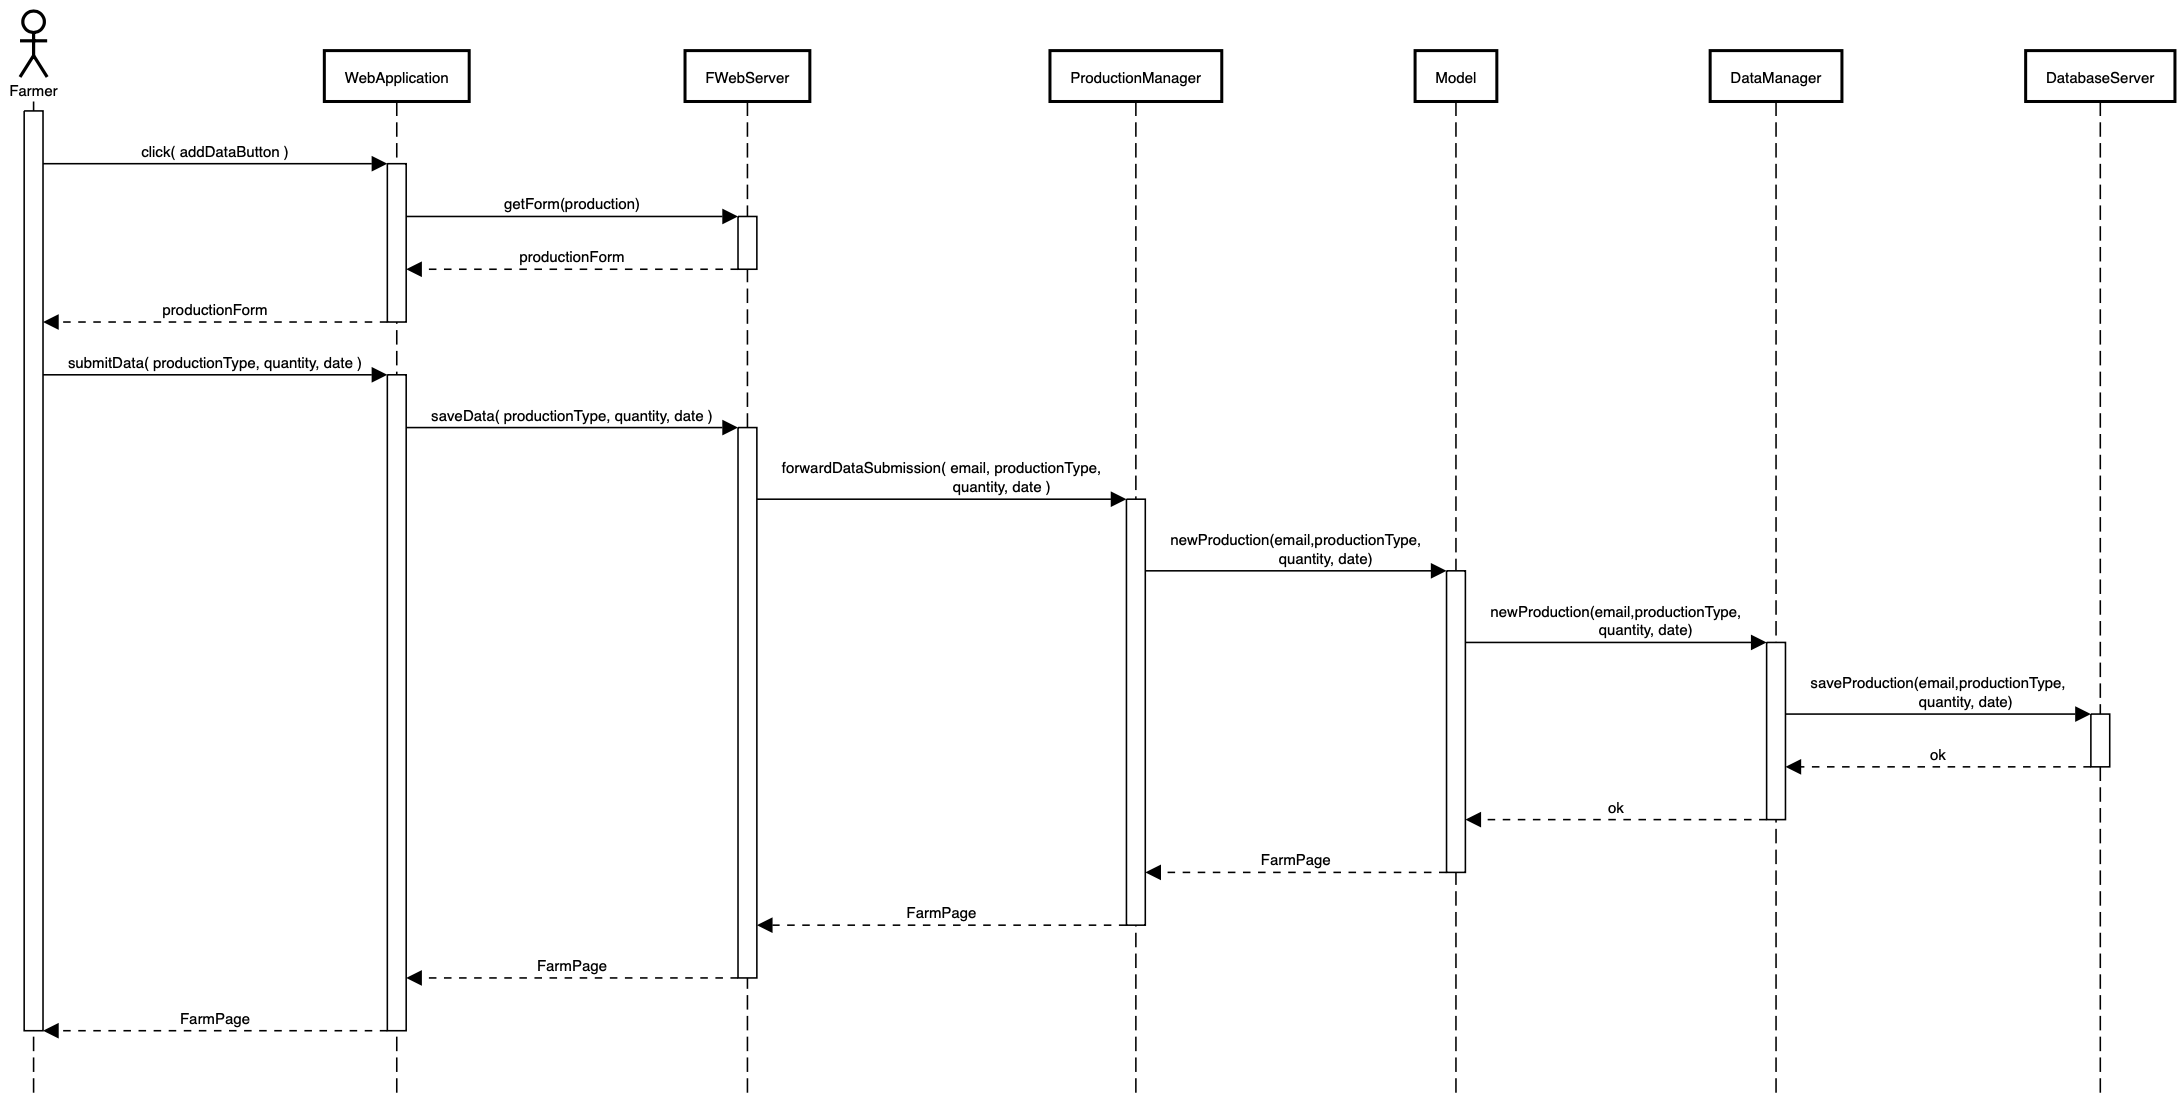
\includegraphics[width=0.7\textwidth]{sequence/addData-2.png}
        \caption{\emph{Submit production data} sequence diagram}
        \label{fig:sequence4}
        \end{center}
    \end{figure}
    \item \textbf{map visualization}\\
    Here is shown how the system provides the visualization of the map to the user, with different level of visibility based on their permission.
        \begin{itemize}
            \item the user is a farmer: the Model contruct the object that rapresenting the map filled with all the farms saved in the system and only the type of production that are producted in it.
            \item the user is a policy maker: the Model contruct the map object with the farms located on it with basic production data and the evaluetion of it.
        \end{itemize}
    From the Map page is possible, by a click on a specific button, for policy maker to evaluate a farm.
    \begin{figure}[H]
        \begin{center}
        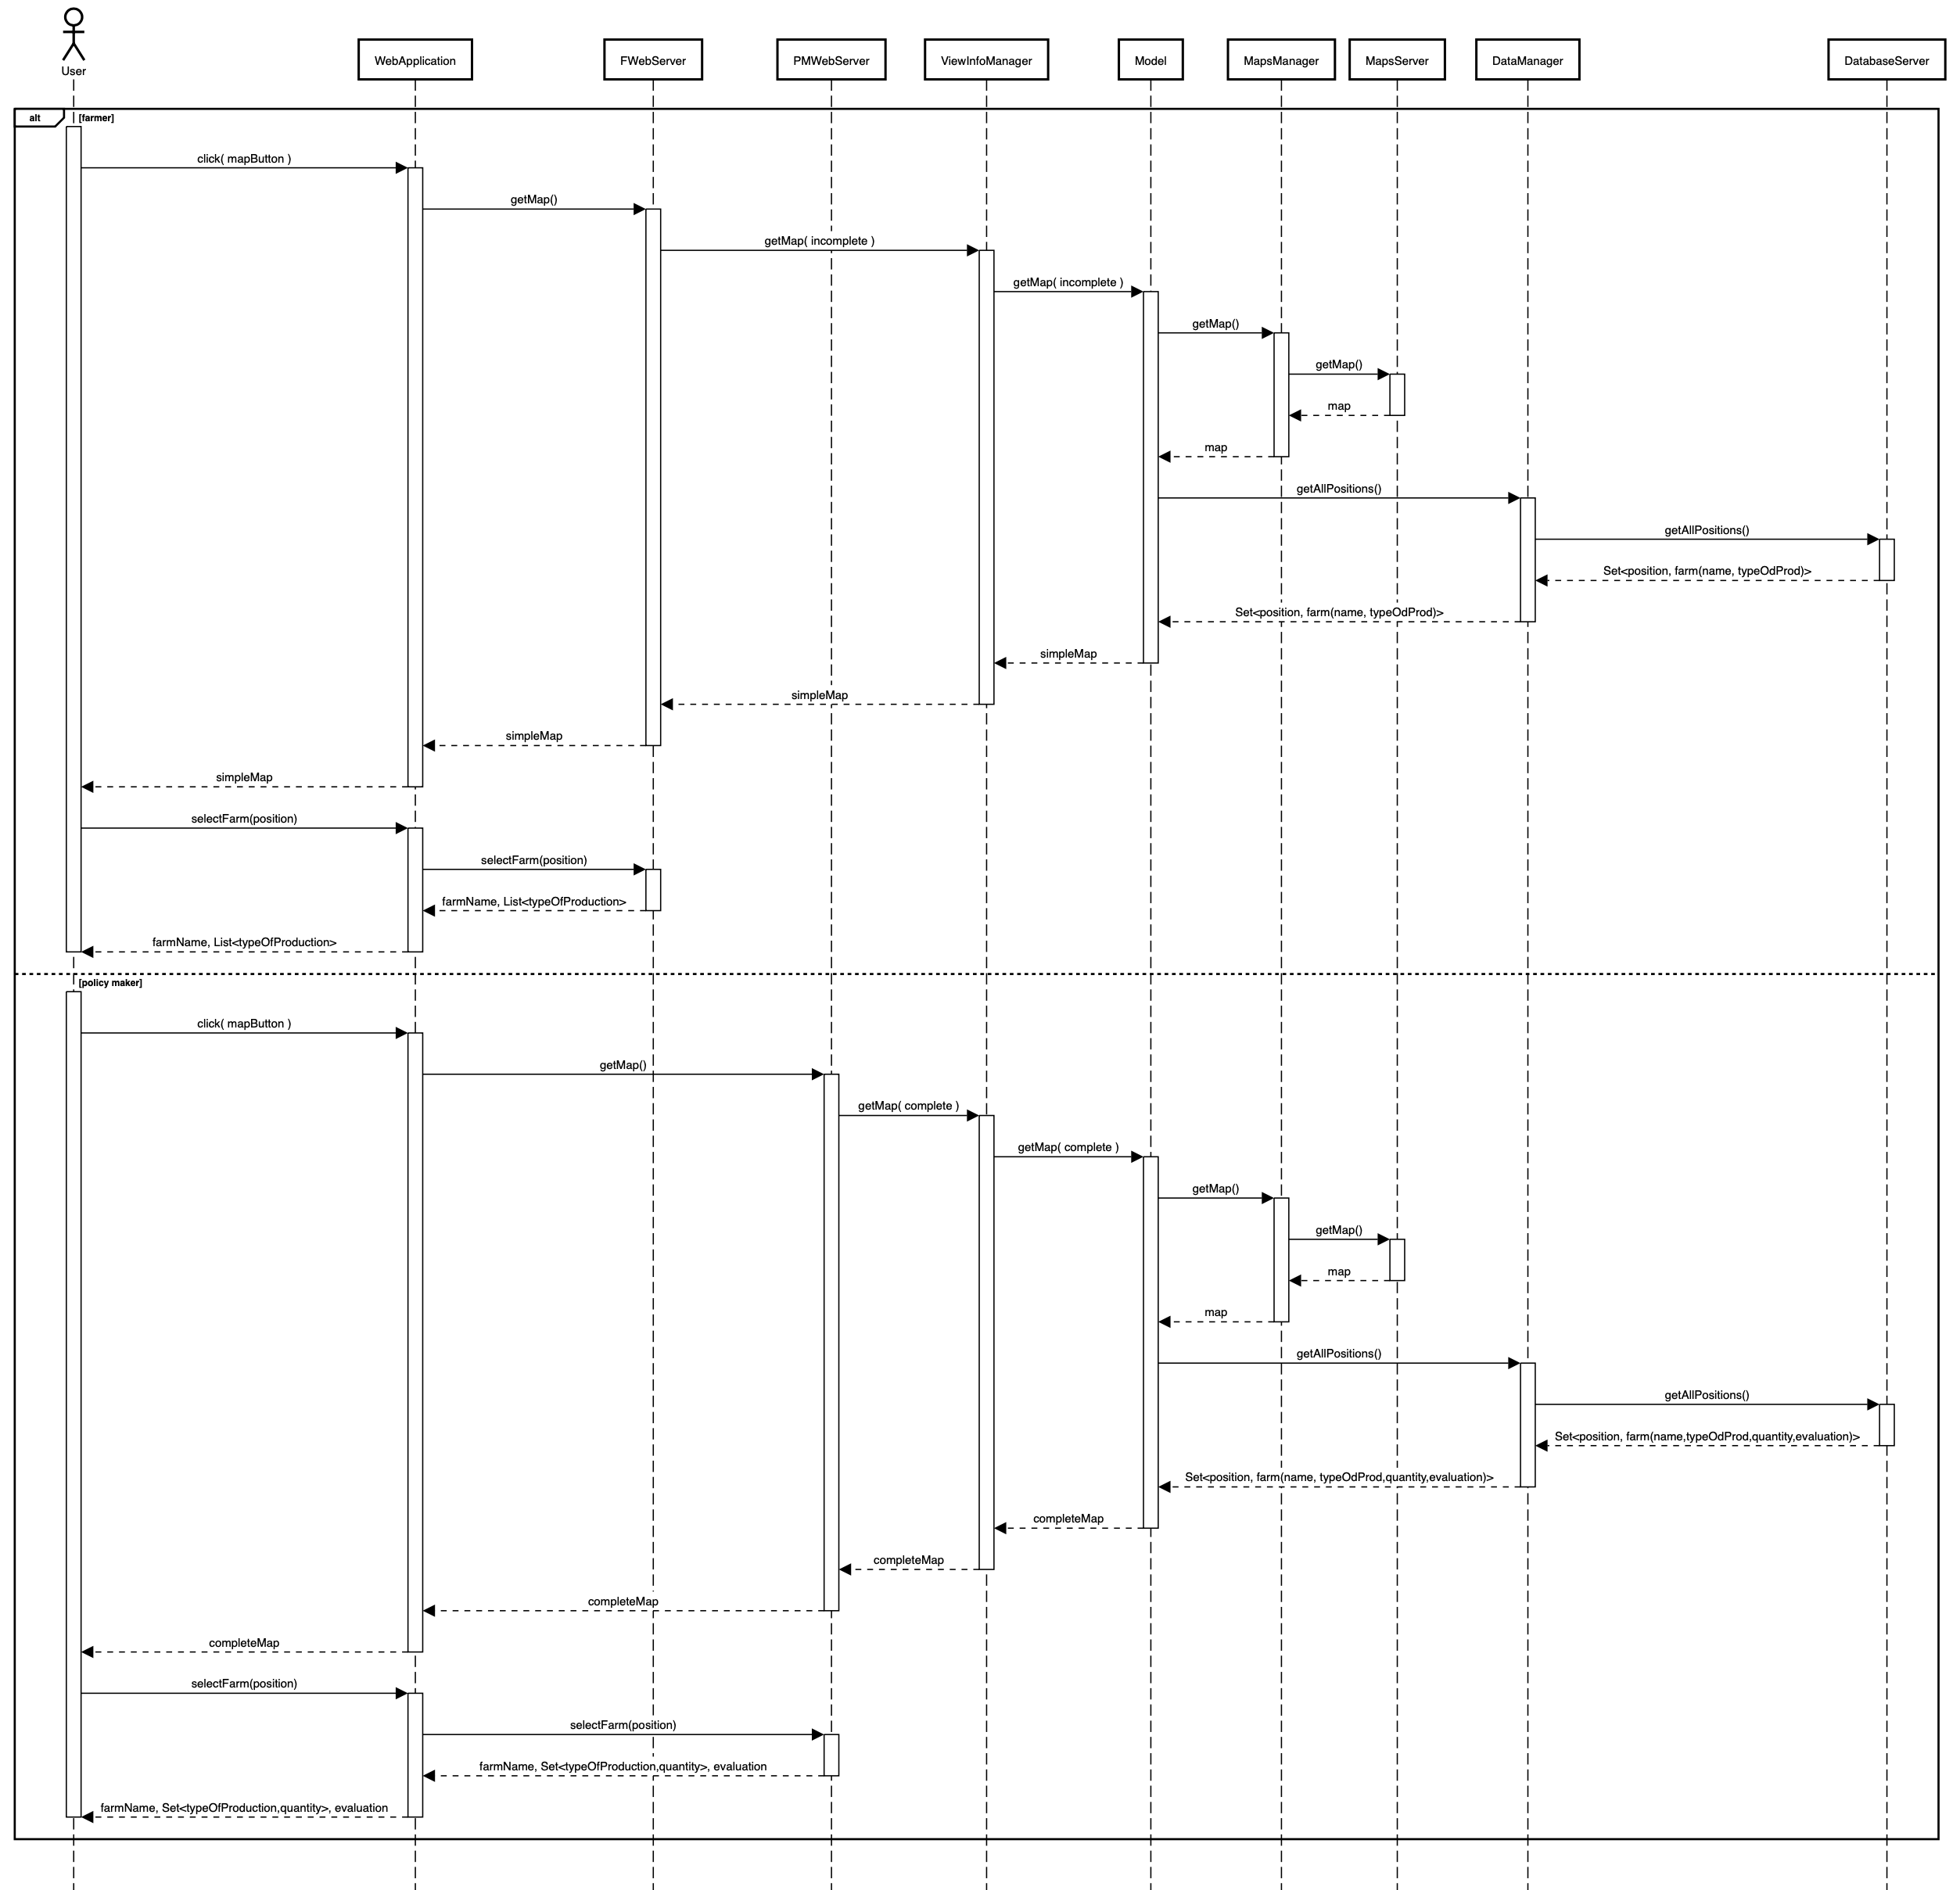
\includegraphics[width=0.7\textwidth]{sequence/viewMap.png}
        \caption{\emph{Visualize map} sequence diagram}
        \label{fig:sequence5}
        \end{center}
    \end{figure}
    \item \textbf{policy maker makes an evaluation}\\
    This diagram describes the process of evaluation a farmer by a policy maker. At first, when the day of the month in wich the evaluation must be done, the policy maker select from the map the farm that he wants to evaluate and he clicks on the 'Evaluate' button. His Web Server provides him the form to fill with the results of the evaluation, with already the addresse attached. When this notification is submitted by the policy maker, his web server forward it to the notification manager that deal with the enrollment of the result in the database and also send it to the farmer evaluated.
    \begin{figure}[H]
        \begin{center}
        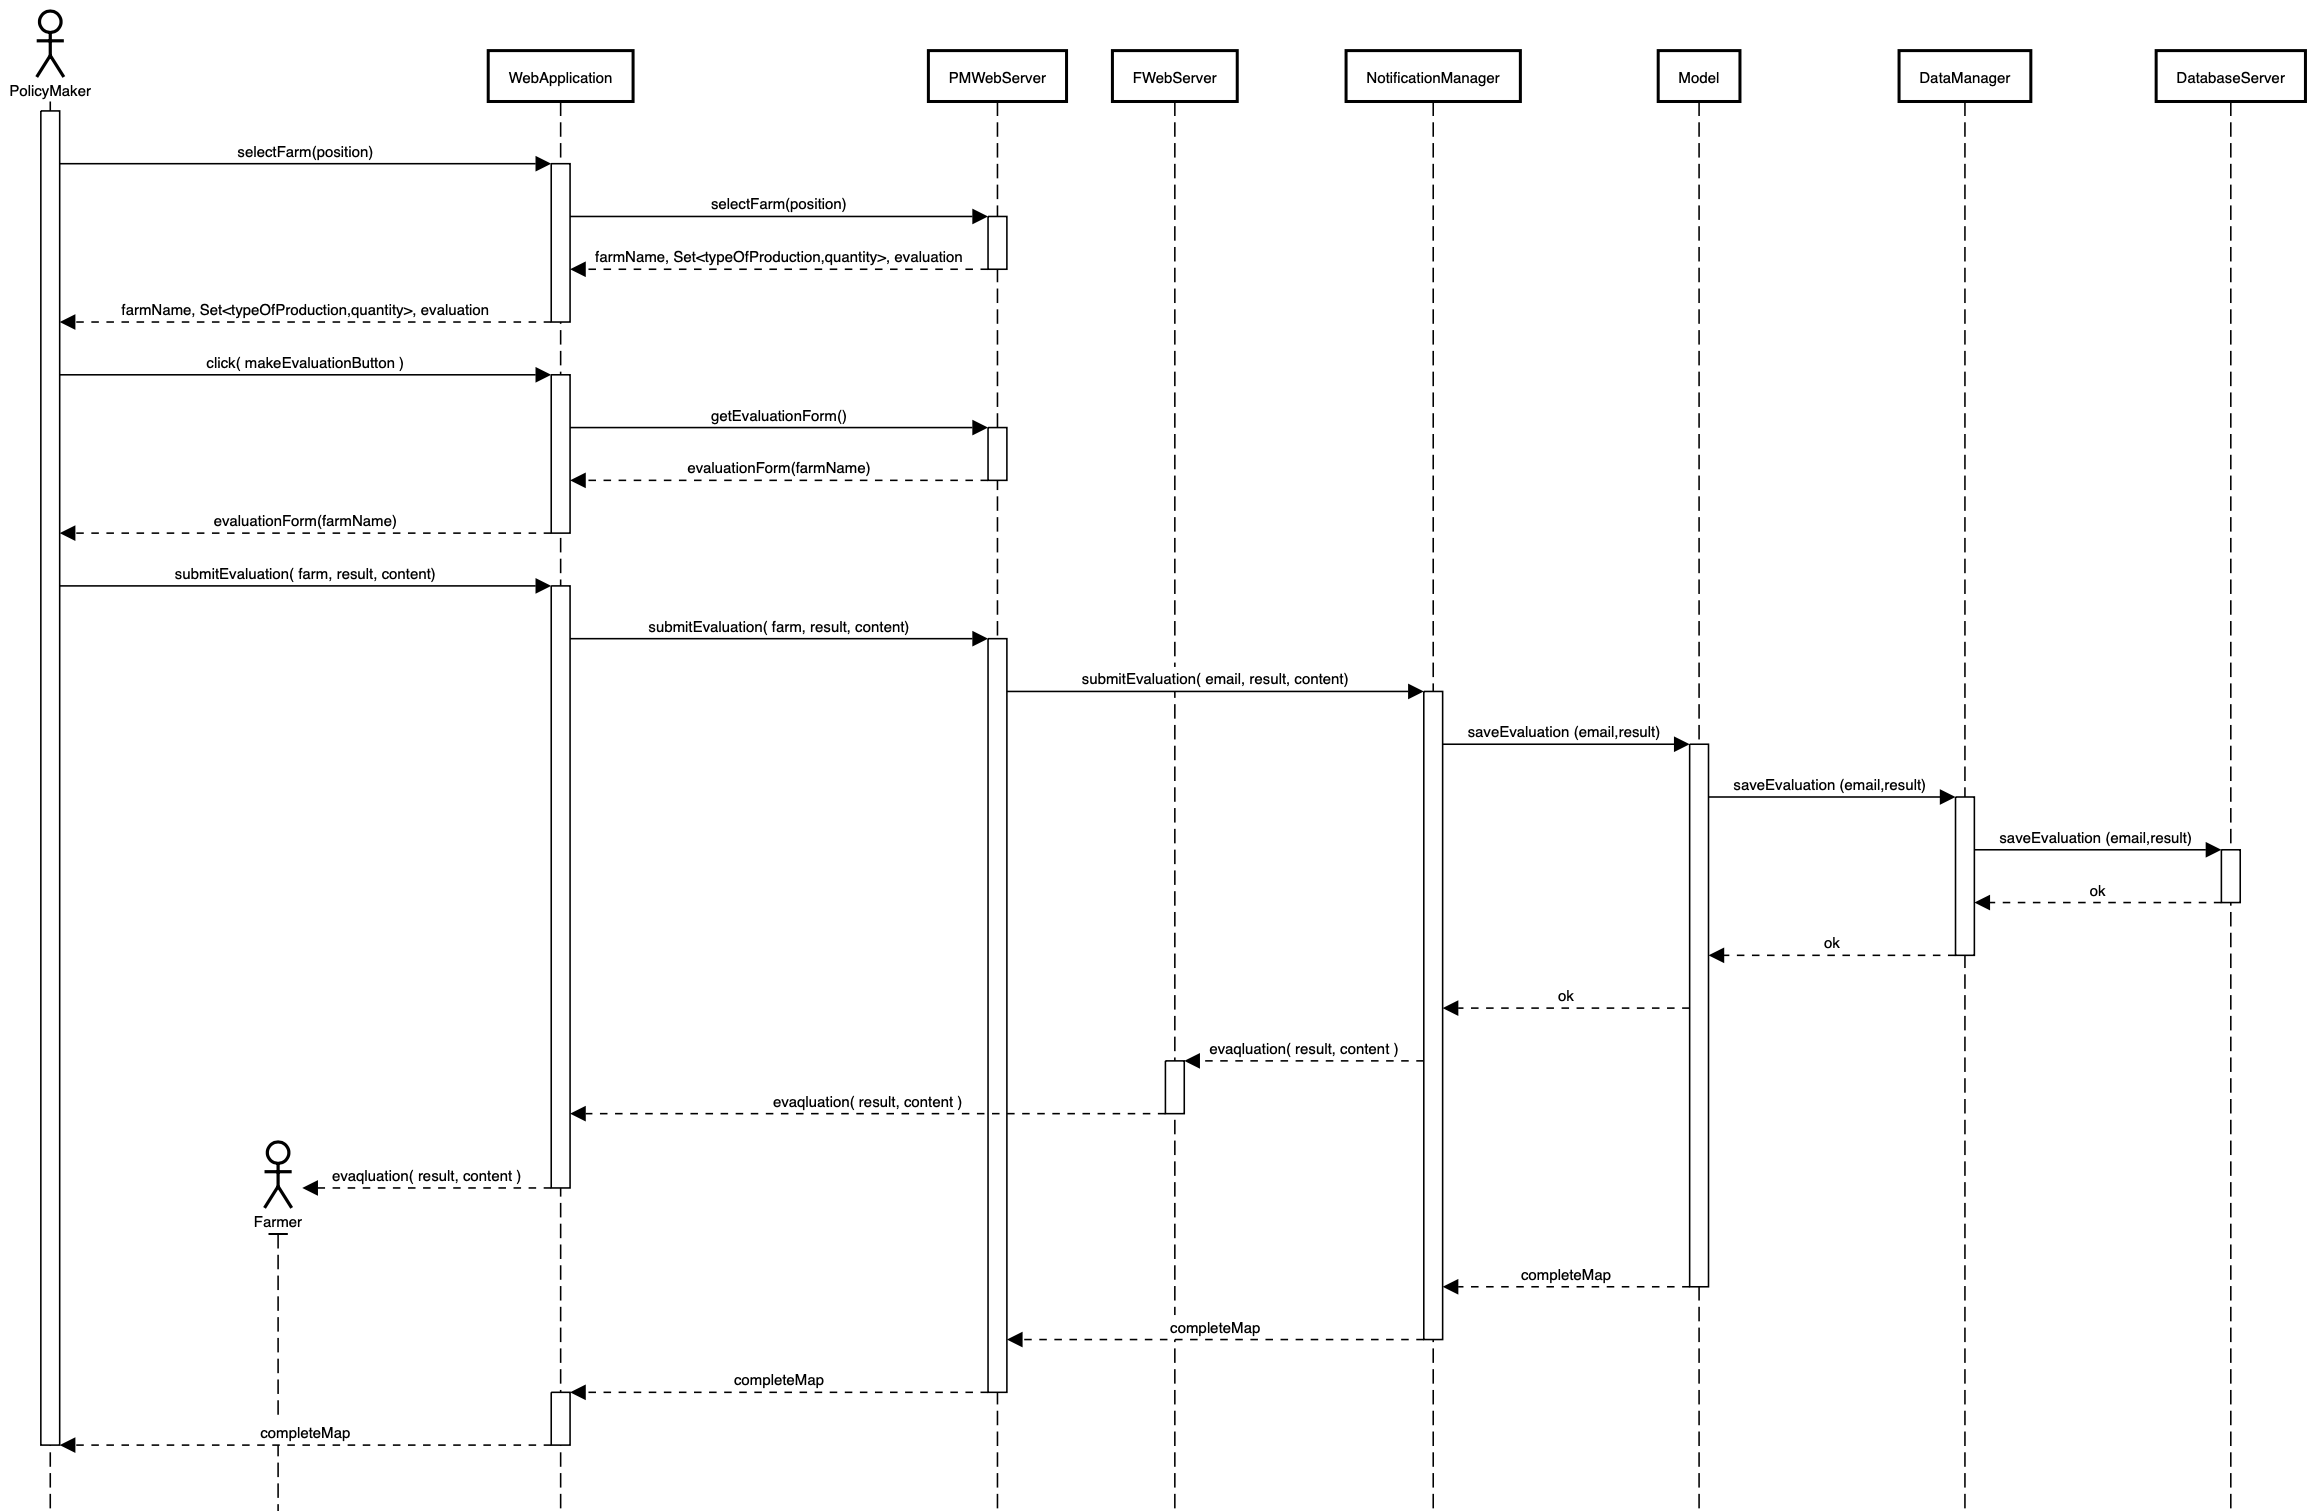
\includegraphics[width=0.7\textwidth]{sequence/updateMap.png}
        \caption{\emph{Make evaluation} sequence diagram}
        \label{fig:sequence6}
        \end{center}
    \end{figure}
    \item \textbf{farm's page visualization}\\
    This functionality is avaiilable for both users, the only differences are:
    \begin{itemize}
        \item a farmer has only a button on his home page that he clicks when wants to visualize his \textbf{own} farm page
        \item a policy maker has a form on which he writes the name of the farm he wants to visualize and pressing enter sends the request to the web application
        \item for the first user the received web page will have a button for the notification visualization and the buttons for the creation of  help and advice notification
    \end{itemize}
    After received the request, the web application sends it to the view info manager (by the user's server), that collects all the data from the model. The last component gets from the right database all the data to generate all the object rapresenting the page content:
    \begin{itemize}
        \item from the application database gets the farm basic information, such as name and surname of the farm's owner, the farm name, the email and the position (as coordinates)
        \item also from the application database it gets the production's information whith which create a set having as key the date and as value another key-value structure containing for each type of production the quantity crop 
        \item the third request to the application database is the one to get the sensors data, that these dispositives put automatically in the database and always related to a specific day and position (corresponding to the farm on which they work)
        \item it asks to the external system to retreive the weather information from the day of the request and all the ones befor in the position on the farm. This information are stored in a database specific of this system
    \end{itemize}
    After the model creates the structure for all the content of the page, forward them to the view info manager to the user's server and then the web application that will provide the visualization of these data.
    \begin{figure}[H]
        \begin{center}
        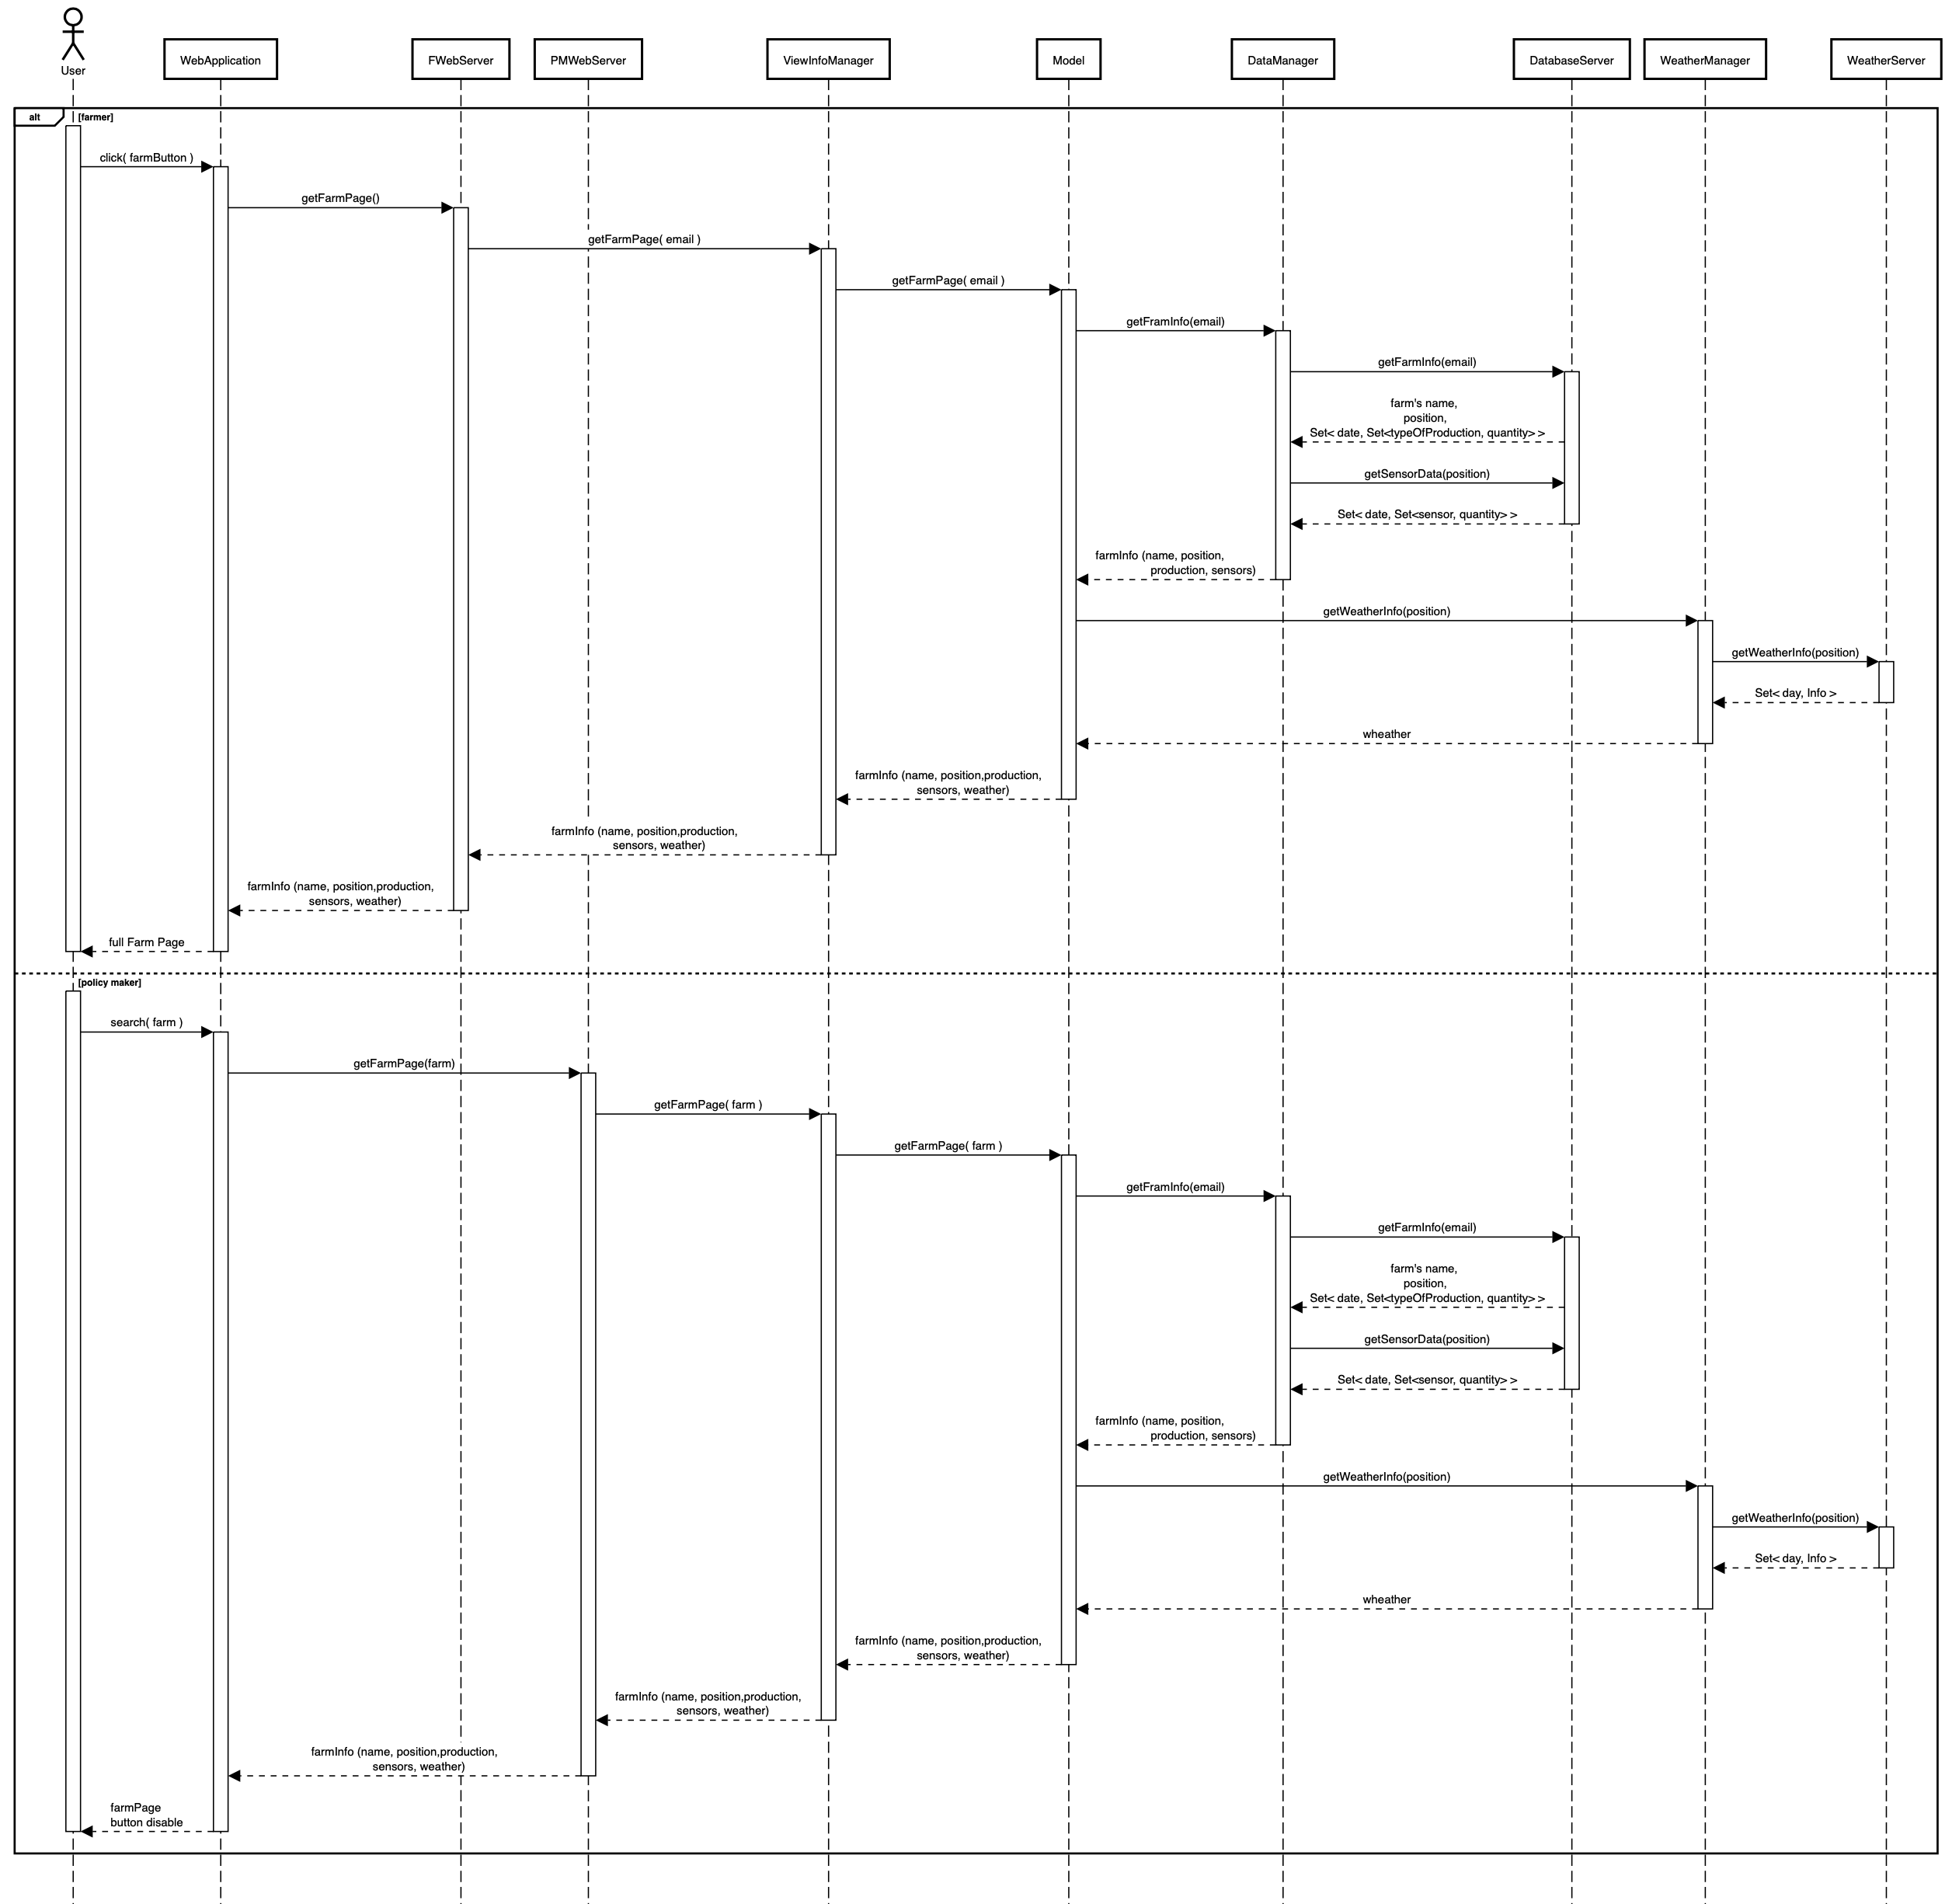
\includegraphics[width=0.7\textwidth]{sequence/farmPage.png}
        \caption{\emph{Visualize farm page} sequence diagram}
        \label{fig:sequence7}
        \end{center}
    \end{figure}
    \item \textbf{notification submittion}\\
    Different kind of notification can be sent in the system.
    \begin{itemize}
        \item advice: a farmer can select the advice button from his farm's page. He just have to select the type of production on which he wants to gave an advice and write it in the specific form. Will be the framer's server that will attach on it the references of the writer (the email of the farmer), and the date and time on which he submit the advice, before saving it in the database. Before push it in the database, the notification manager checks it the sender is a good farmer and if not just discard the notification.
        \item help: a farmer who wants to ask a formal request of help also select the help button on his farm's page. As the notification above he select the type and writes the content of the message, where specify the problem he's dealing with. In this case the notification does not need to be saved in a db but the notification manager selects randomly a policy maker as a recipient of it. 
        \item solution: a policy maker who received a request of help (process described above) can reply to it whith a solution. At first the user have to search the farm ho asks for it, and also all the avices stored in the system database about the type of production on which the problem is specified. Analyzing all these data he can  wrote some advice that should help the farmer with his problem and send him. In the moment when the policy maker selects the help notification on which he wants to respond and then submit it, the web application istantinelly attach the addresse (retreived by the sender of the help selected) and then the notification manager will forward it to him.
    \end{itemize}
    \begin{figure}[H]
        \begin{center}
        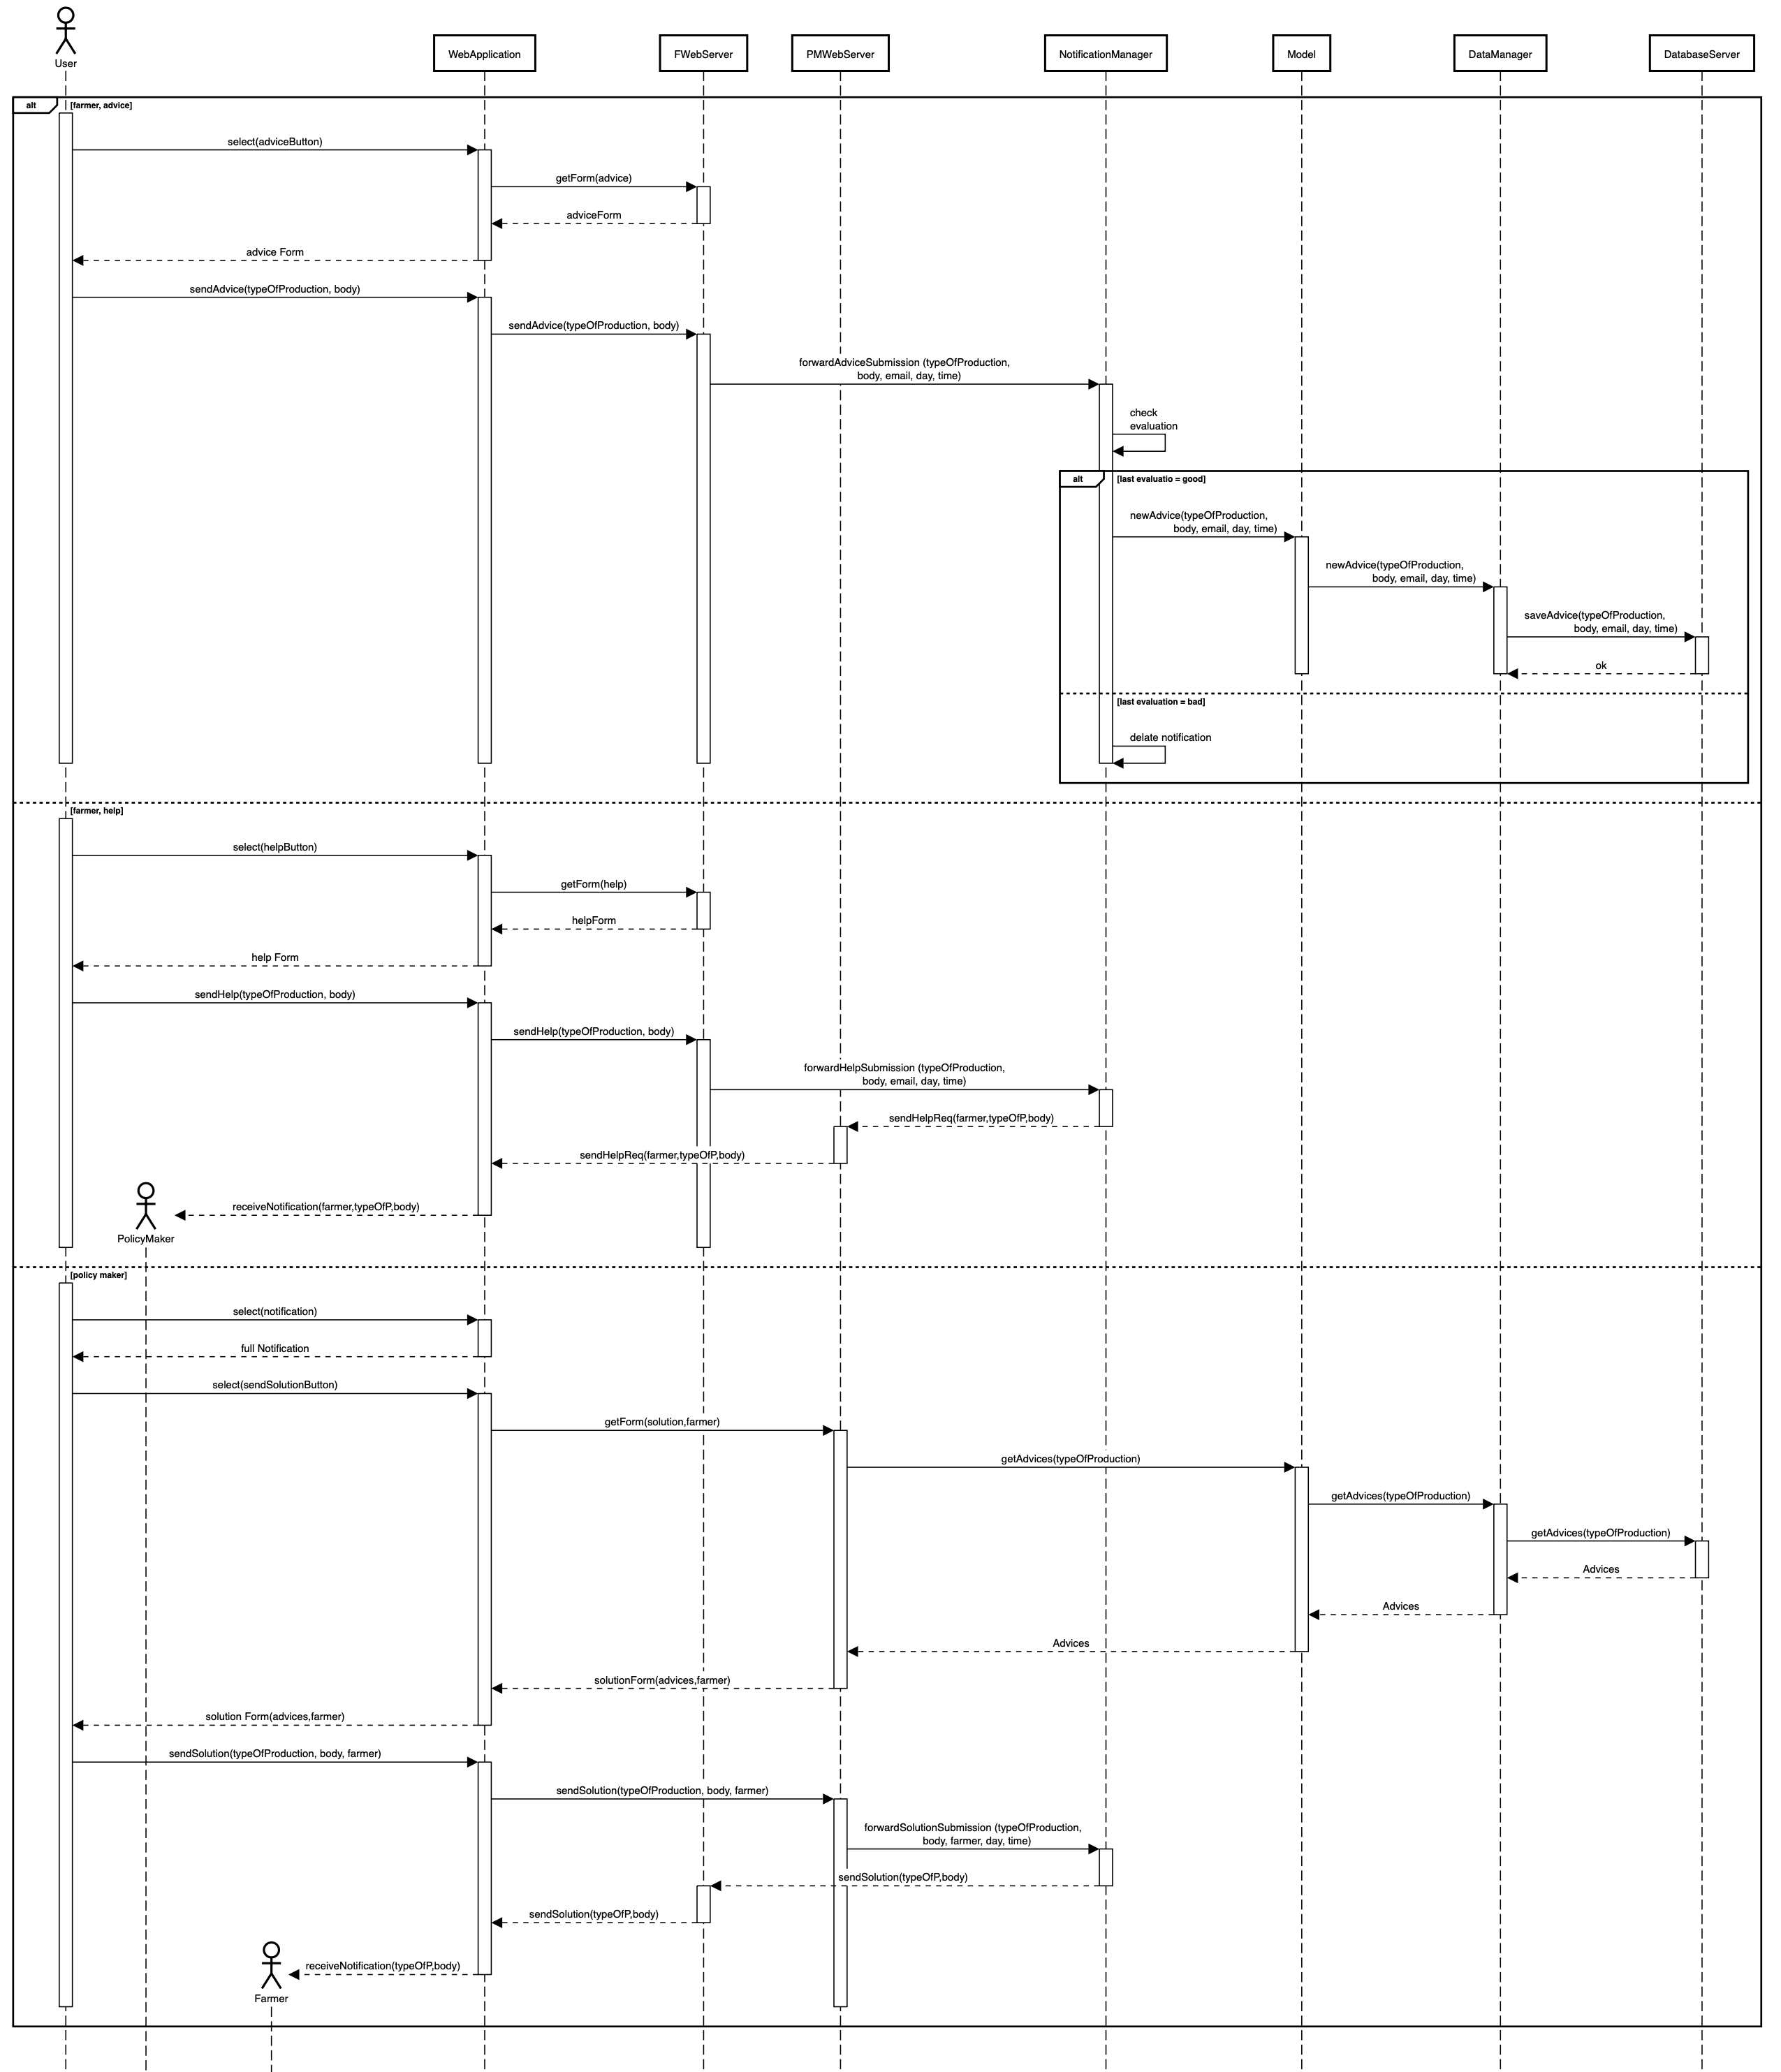
\includegraphics[width=0.7\textwidth]{sequence/sendNotifications.png}
        \caption{\emph{Send notifications} sequence diagram}
        \label{fig:sequence8}
        \end{center}
    \end{figure}
    \item \textbf{notification visualization}\\
    In this sequence is shown how the system provide the visualization of the notifications after a request of a user. For the farmer the process starts on his farm's page, where clicking the bell button send the request, dream server collect from the database all his notification. The model crete with the data the structure to be sent to the web application that provide the list to the user. All the messages are in the web application in that moment, so when he select one of the notifications in the list it provides the full content of it. on the other hand the policy maker to visualize his notifications starts from his home page and clicks on the specific button. The rest of the process is equal as for the farmer.
    \begin{figure}[H]
        \begin{center}
        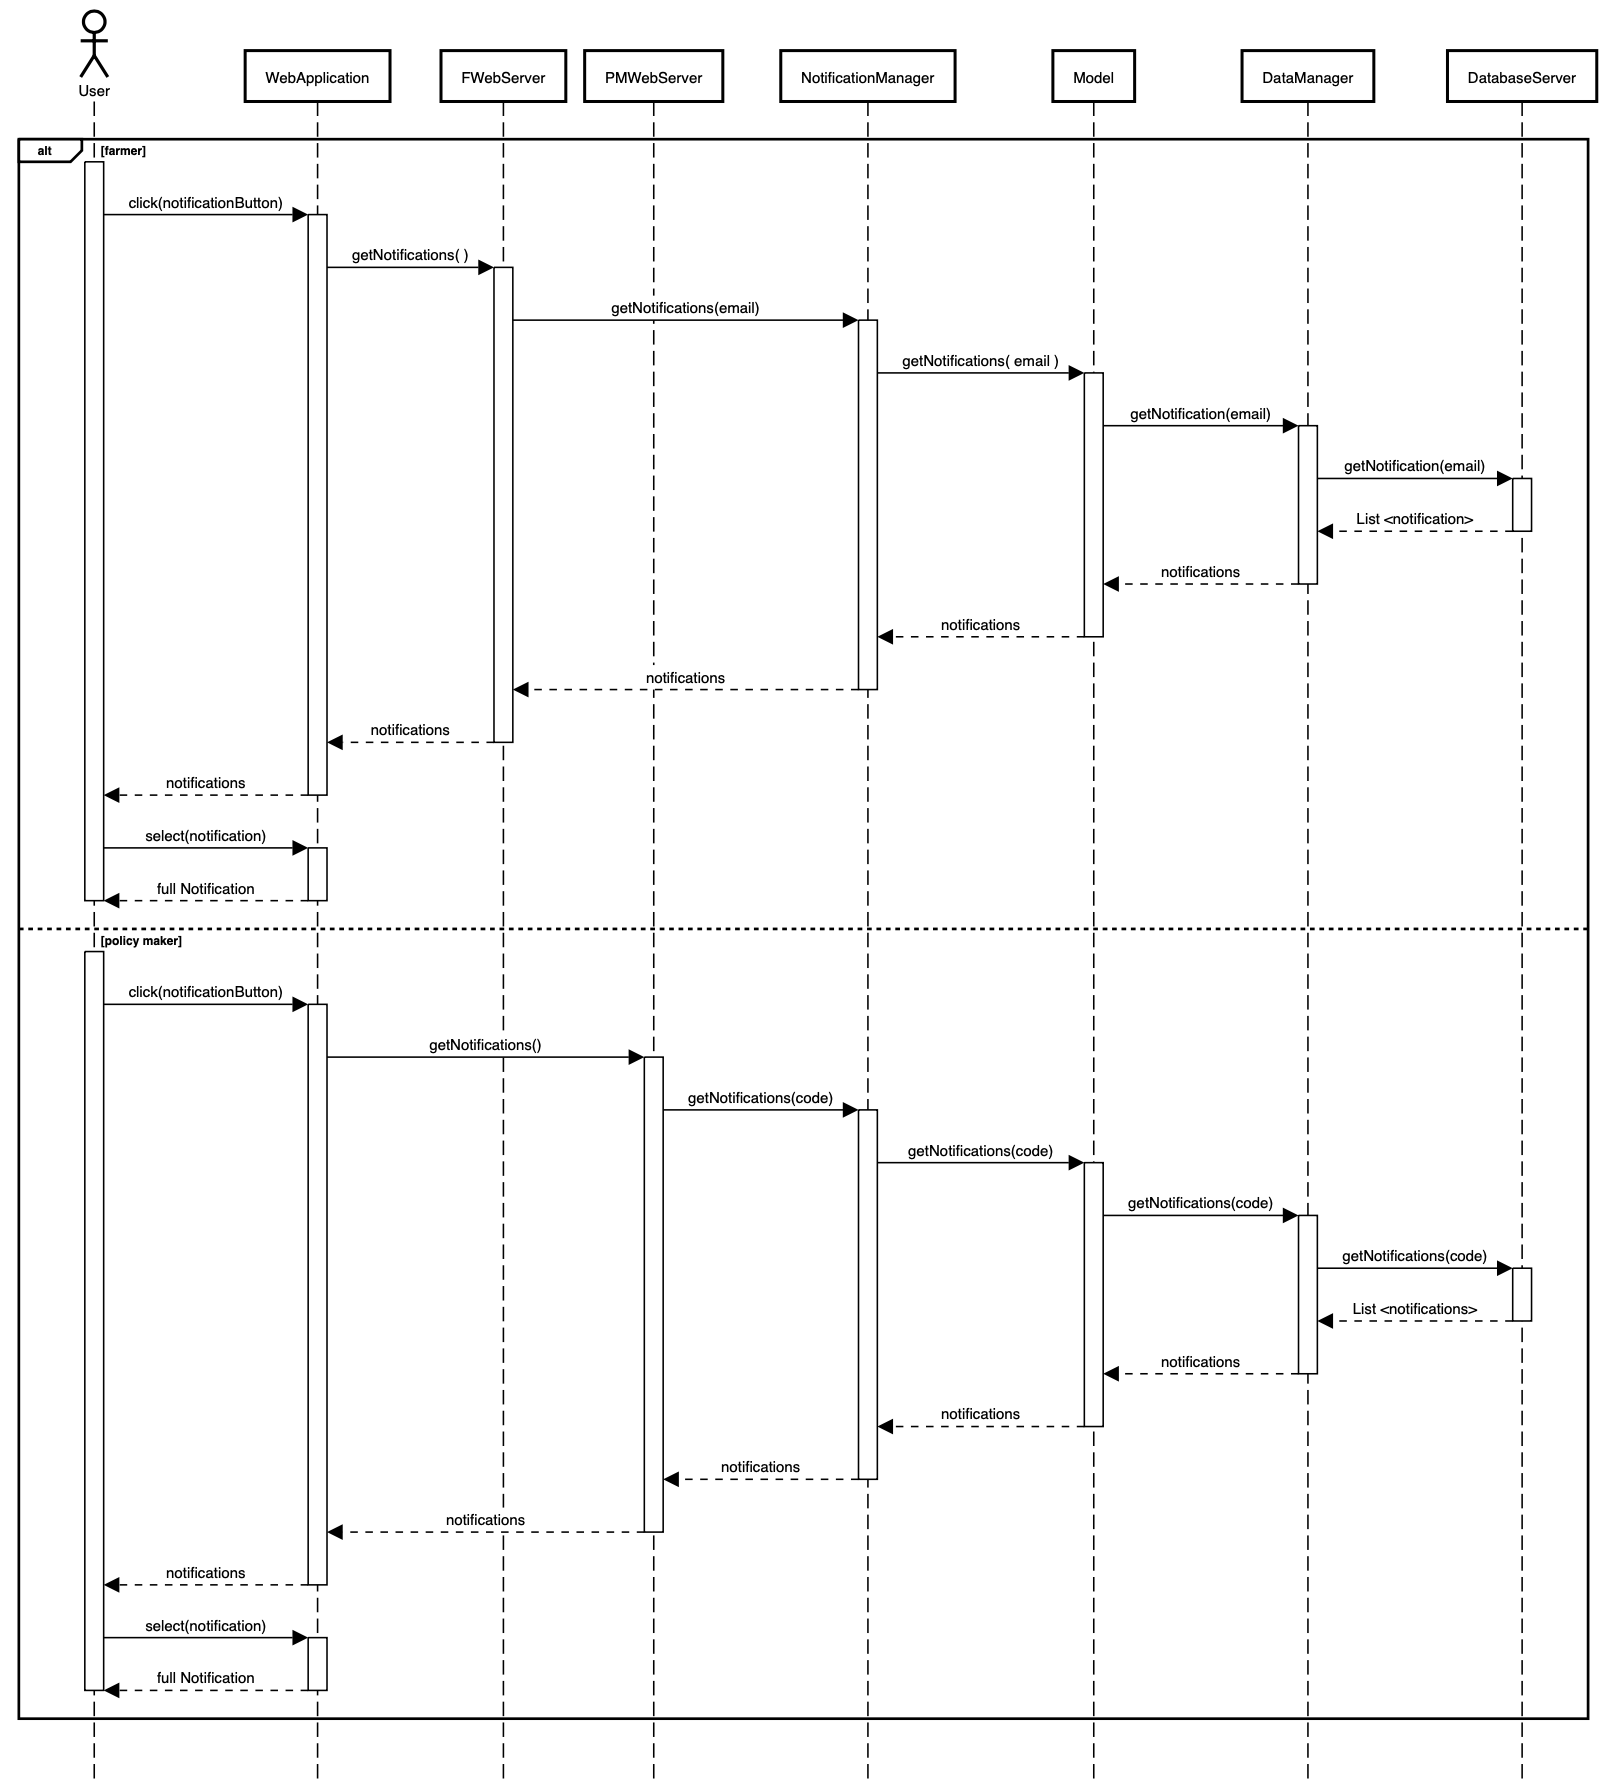
\includegraphics[width=0.7\textwidth]{sequence/viewNotifications.png}
        \caption{\emph{Visualize notifications} sequence diagram}
        \label{fig:sequence9}
        \end{center}
    \end{figure}
    
\end{enumerate}


%---------------------%
\subsection{Component interfaces}
In this section an image (Figure \ref{fig:interfacesView}) of all the interfaces that compose the system is provide. In it is not only specified the name of them but also all the methods provided by the components they implements. To follow there is a brief explenation of each one. All the methods present in the sequence diagrams must be present here. 

\begin{adjustbox}{angle=90,center,caption=\emph{Interfaces} view,nofloat=figure}
    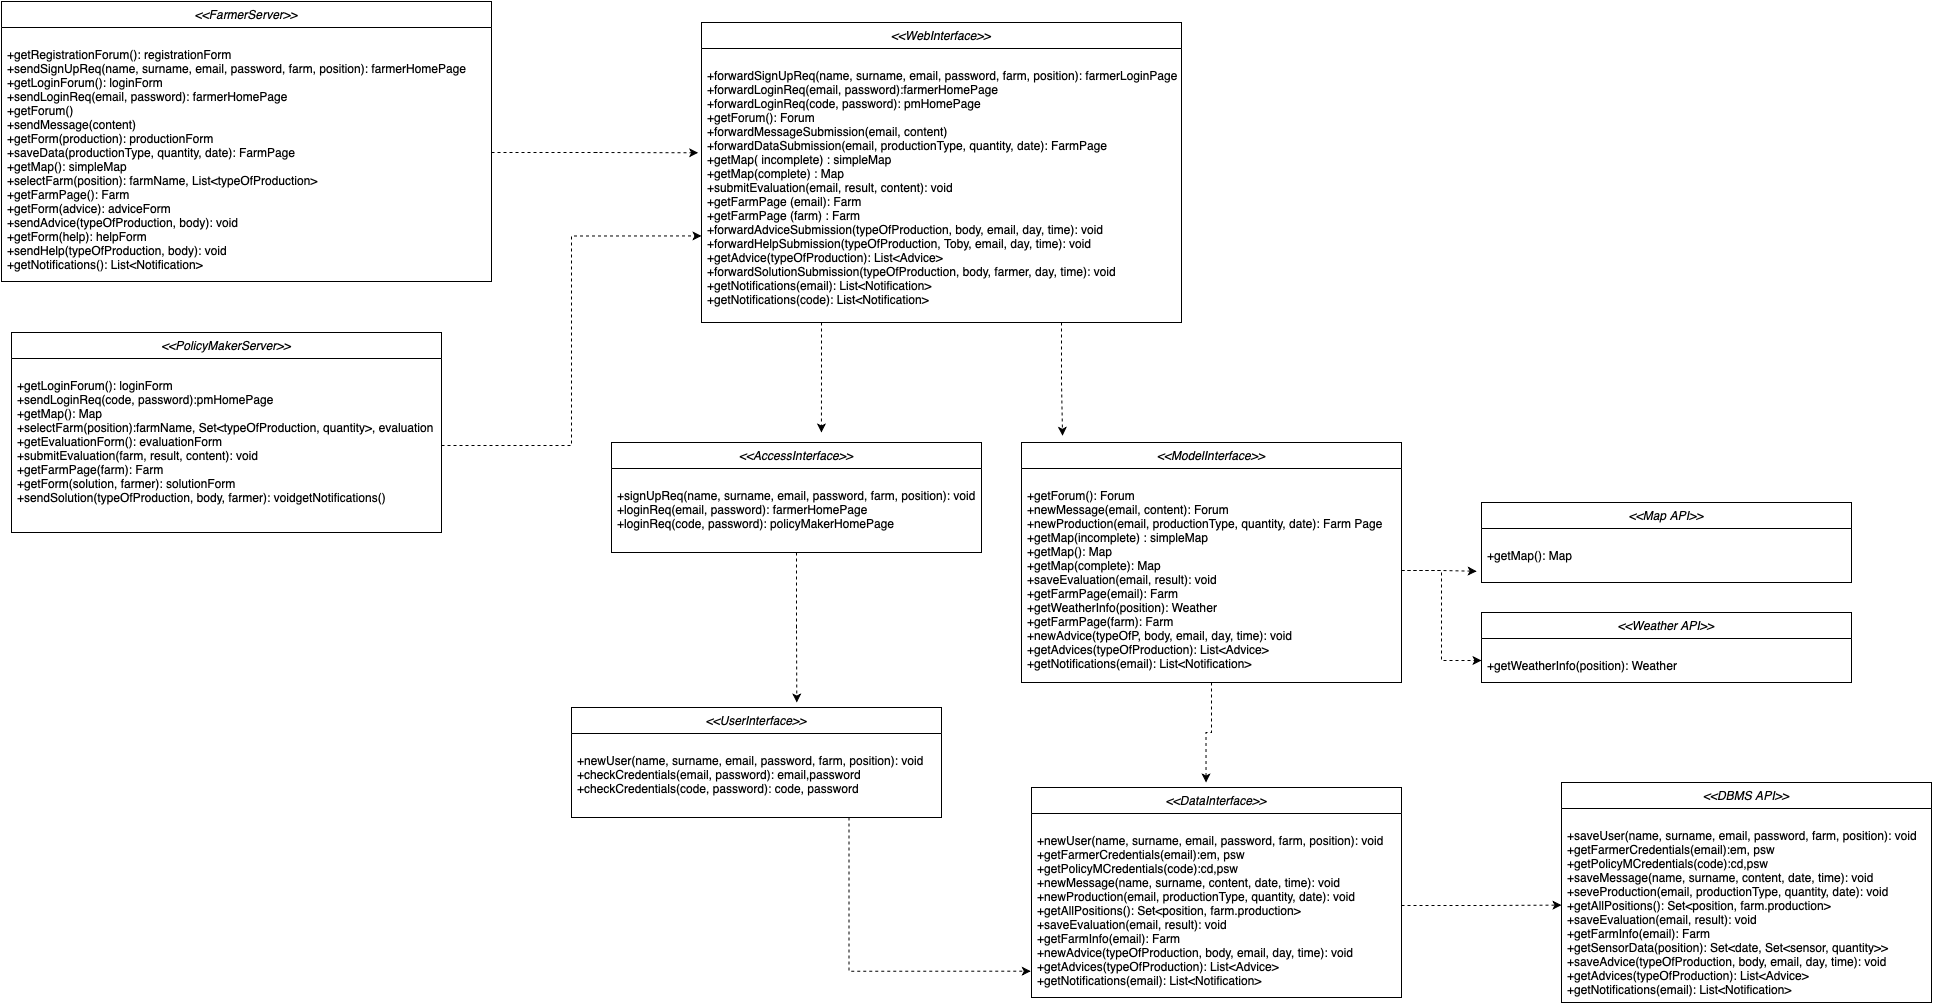
\includegraphics[width=1.6\linewidth]{images/Interfaces.png}
    \label{fig:interfacesView}
\end{adjustbox}



\begin{itemize}
    \item \textbf{Farmer Server Interface}: this interfaces is specific for the farmer user. Its main pourpose is to connected the Web Application with the Server of the farmer; in order to do that its methods are implemented by the web aplication. In the case in wich the data required by the user are already loaded in the client server, it will not forward the request to the server system, the data will be provided immediatelly. On the other hand, for example when data required are stored in the db of the application, the request will be forwarded to the system (with the following components, as specified in the section 2.2)
    \item \textbf{Policy Maker Interface}: this interface works as the previous one, with the difference that the user that needs these functionality is a policy maker; the component that implements its method is also the web application, but comunicates with the policy maker web server.
    \item \textbf{Web Interface}: this interface have the main pourpose of forwarding the user request to the right component of the system. The components that have its exposed methods are the farmer web server and the policy maker web server.   
    \item \textbf{Access Interface}: in this case the interface is inside the system server. Its main scope is to provide methods for the authentication or registration phase; to reach its goal the component that implements its method is the access manager, that also forward the request to the next right component: one for the registration and one for the authentication.
    \item \textbf{User Interface}: with the aim of ability the access to a user, this itervace provide to the register service and authentication service components the method to comunicate with the model, and retreive the information to check the credentials or save the new ones.
    \item \textbf{Model Interface}: this interface it's in the core of the system. It let components as view info manager, notification manager, production manager and forum manager comunicate with the model, and also retreive the object to reply to a user with the information required. These data could be already in the model or that component will retreive them from the db or the external system. This interface provide also methods for the model to ask to the maps manager and weather manager some data.  
    \item \textbf{Data Interface}: with this interface the model has all the methods to request the data needed from the database, forwarding it to the data manager component. 
    \item \textbf{DBMS API}: here is the final step of the data reaching, where the methods of this interface are used to translate the request of the system in a db language (as SQL).
    \item \textbf{Map API}: this interface is used when data from the map external syetm are required, so with its methos let the maps manager comunicate with the maps server.
    \item \textbf{Weather API}: the same as the one above but with the weather information, so its exposed methods are implemented by the weather manager that comunicates with the weather server.
\end{itemize}
%---------------------%
\subsection{Logical description of data}



%---------------------%
\subsection{Architectural styles and patterns}

\subsubsection{Server-Client architecture}
As specified in section 2.2 the system is develop over a client-server architecture. It is a computing model in which the server hosts, delivers and manages most of the resources and services to be consumed by the client. This type of architecture has one or more client computers connected to a central server over a network or internet connection. This system shares computing resources. Server-client architecture is also known as a networking computing model or client-server network because all the requests and services are delivered over a network.
\begin{figure}[H]
    \begin{center}
    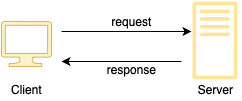
\includegraphics[width=0.5\textwidth]{images/client-server.png}
    \caption{\emph{Server-client} architecture}
    \label{fig:client-server}
    \end{center}
\end{figure}

\subsubsection{Four-tier architecture}
presentation on web application (user browser), logic (web server and dream server)[2] and data on db 

\subsubsection{RESTful architecture}
REST stands for REpresentational State Transfer. REST is a software architectural style that defines the set of rules to be used for creating web services. Web services which follow the REST architectural style are known as RESTful web services. It allows requesting systems to access and manipulate web resources by using a uniform and predefined set of rules. Interaction in REST based systems happen through Internet’s Hypertext Transfer Protocol (HTTP). This protocolo is used not only to retreive data but also generate operation on them in many different forms, such as XML and JSON.

%---------------------%
\subsection{Other design decisions}



%-----------------------------------------------------------%
\newpage
\section{User Interface Design}
In this section there is a complete view of how the web application is going to look. 
It includes diagrams that show hot the users can navigate in the user interfaces offered by the aplication.
Its main purpose is to describe in details the mockups that are already presented in the RASD (reference). Therefore it is easier to understand 
the main features that the system offers.


\subsection{UX diagrams}
This subsection focuses on the flow of the windows of the web application, 
both for farmers and policy makers.

\begin{figure}[H]
    \begin{center}
          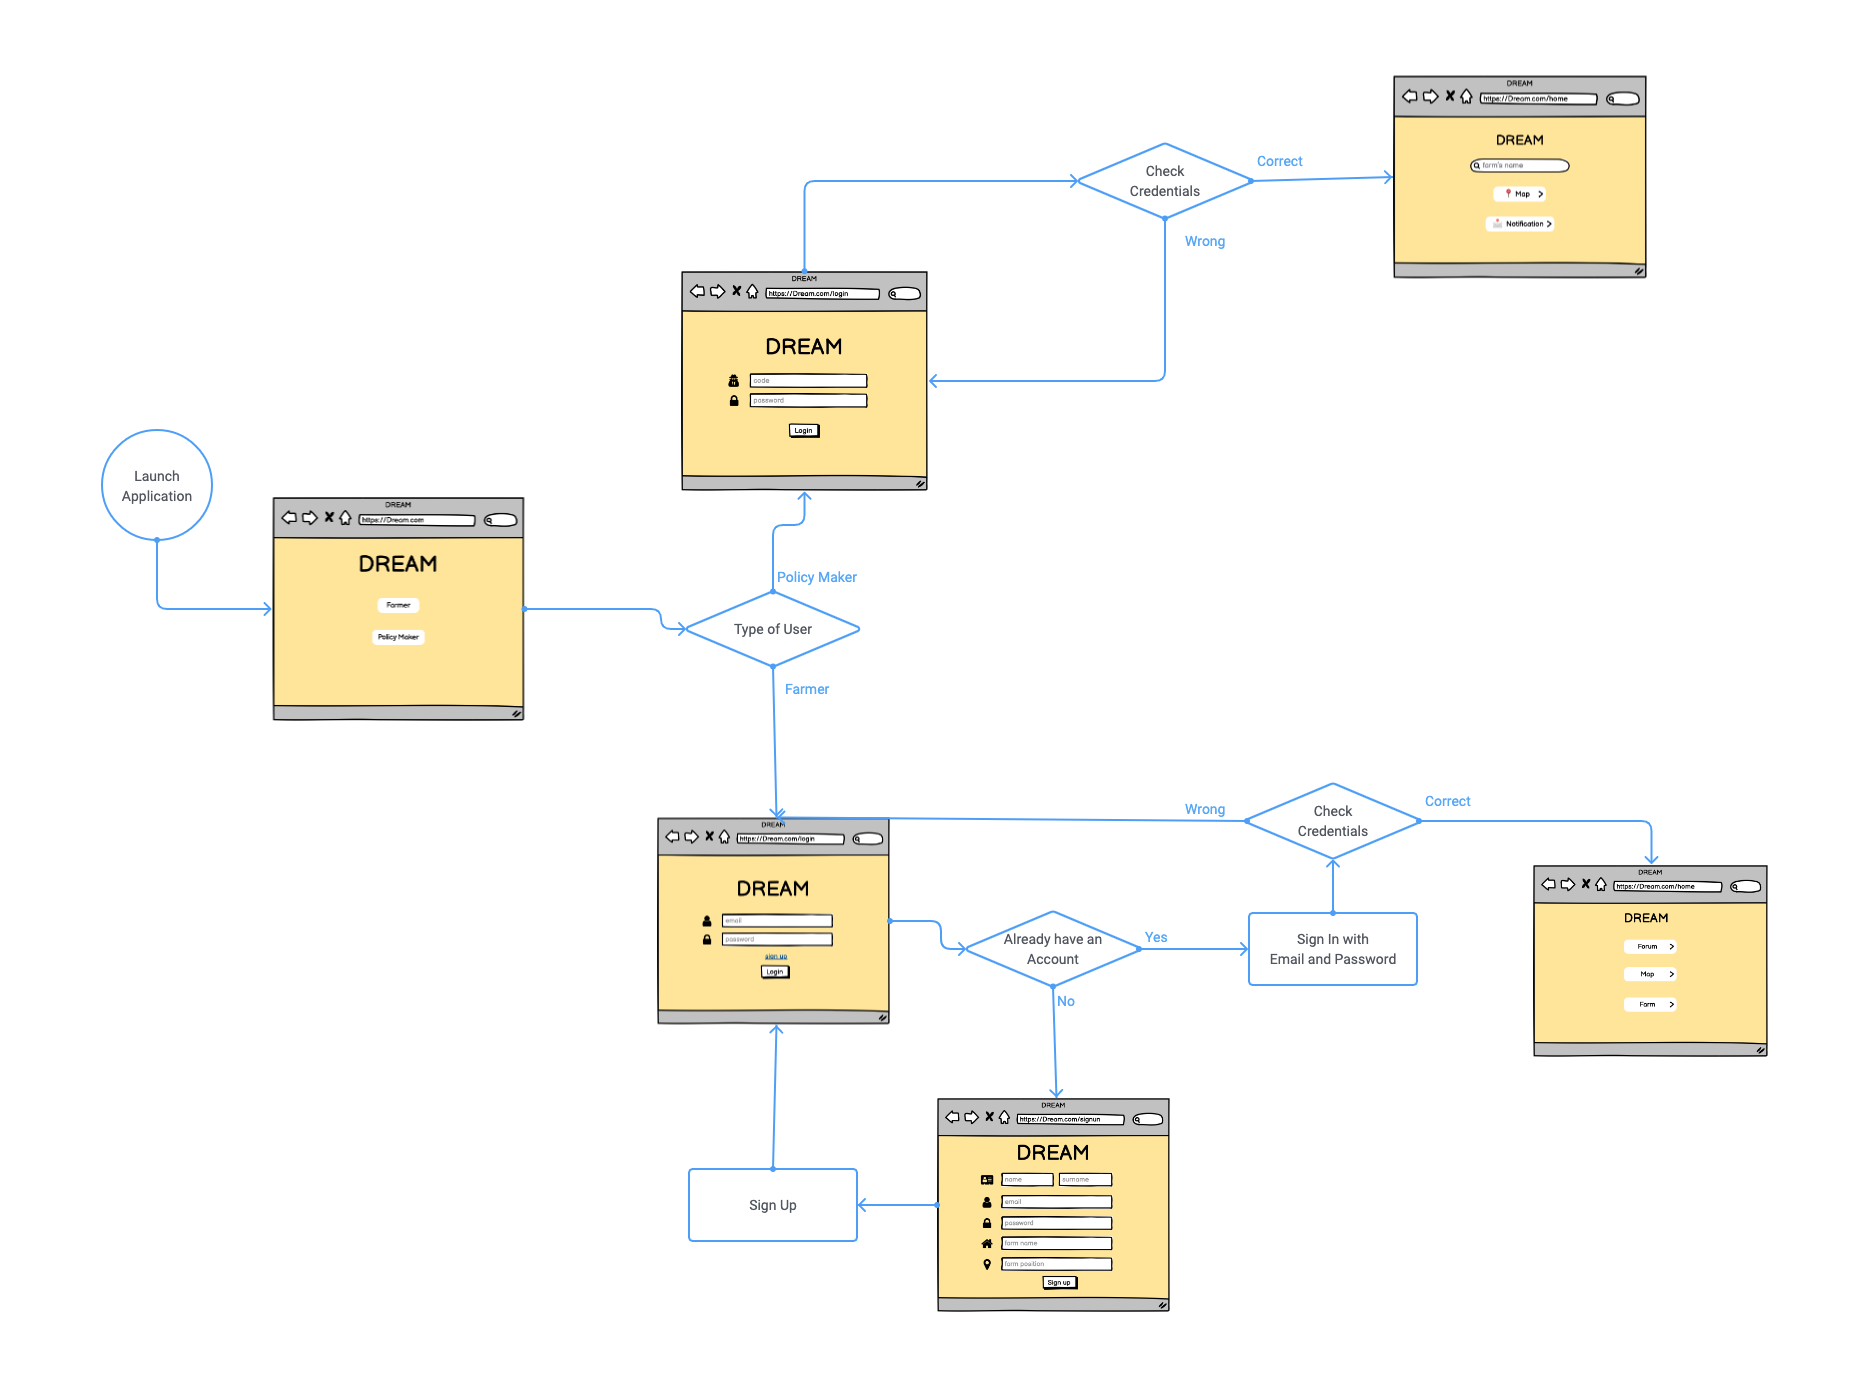
\includegraphics[width=1\textwidth]{images/UXdiagram_login.png}
          \caption{Sign Up \& Sign In}
    \end{center}
\end{figure}

\begin{figure}[H]
    \begin{center}
          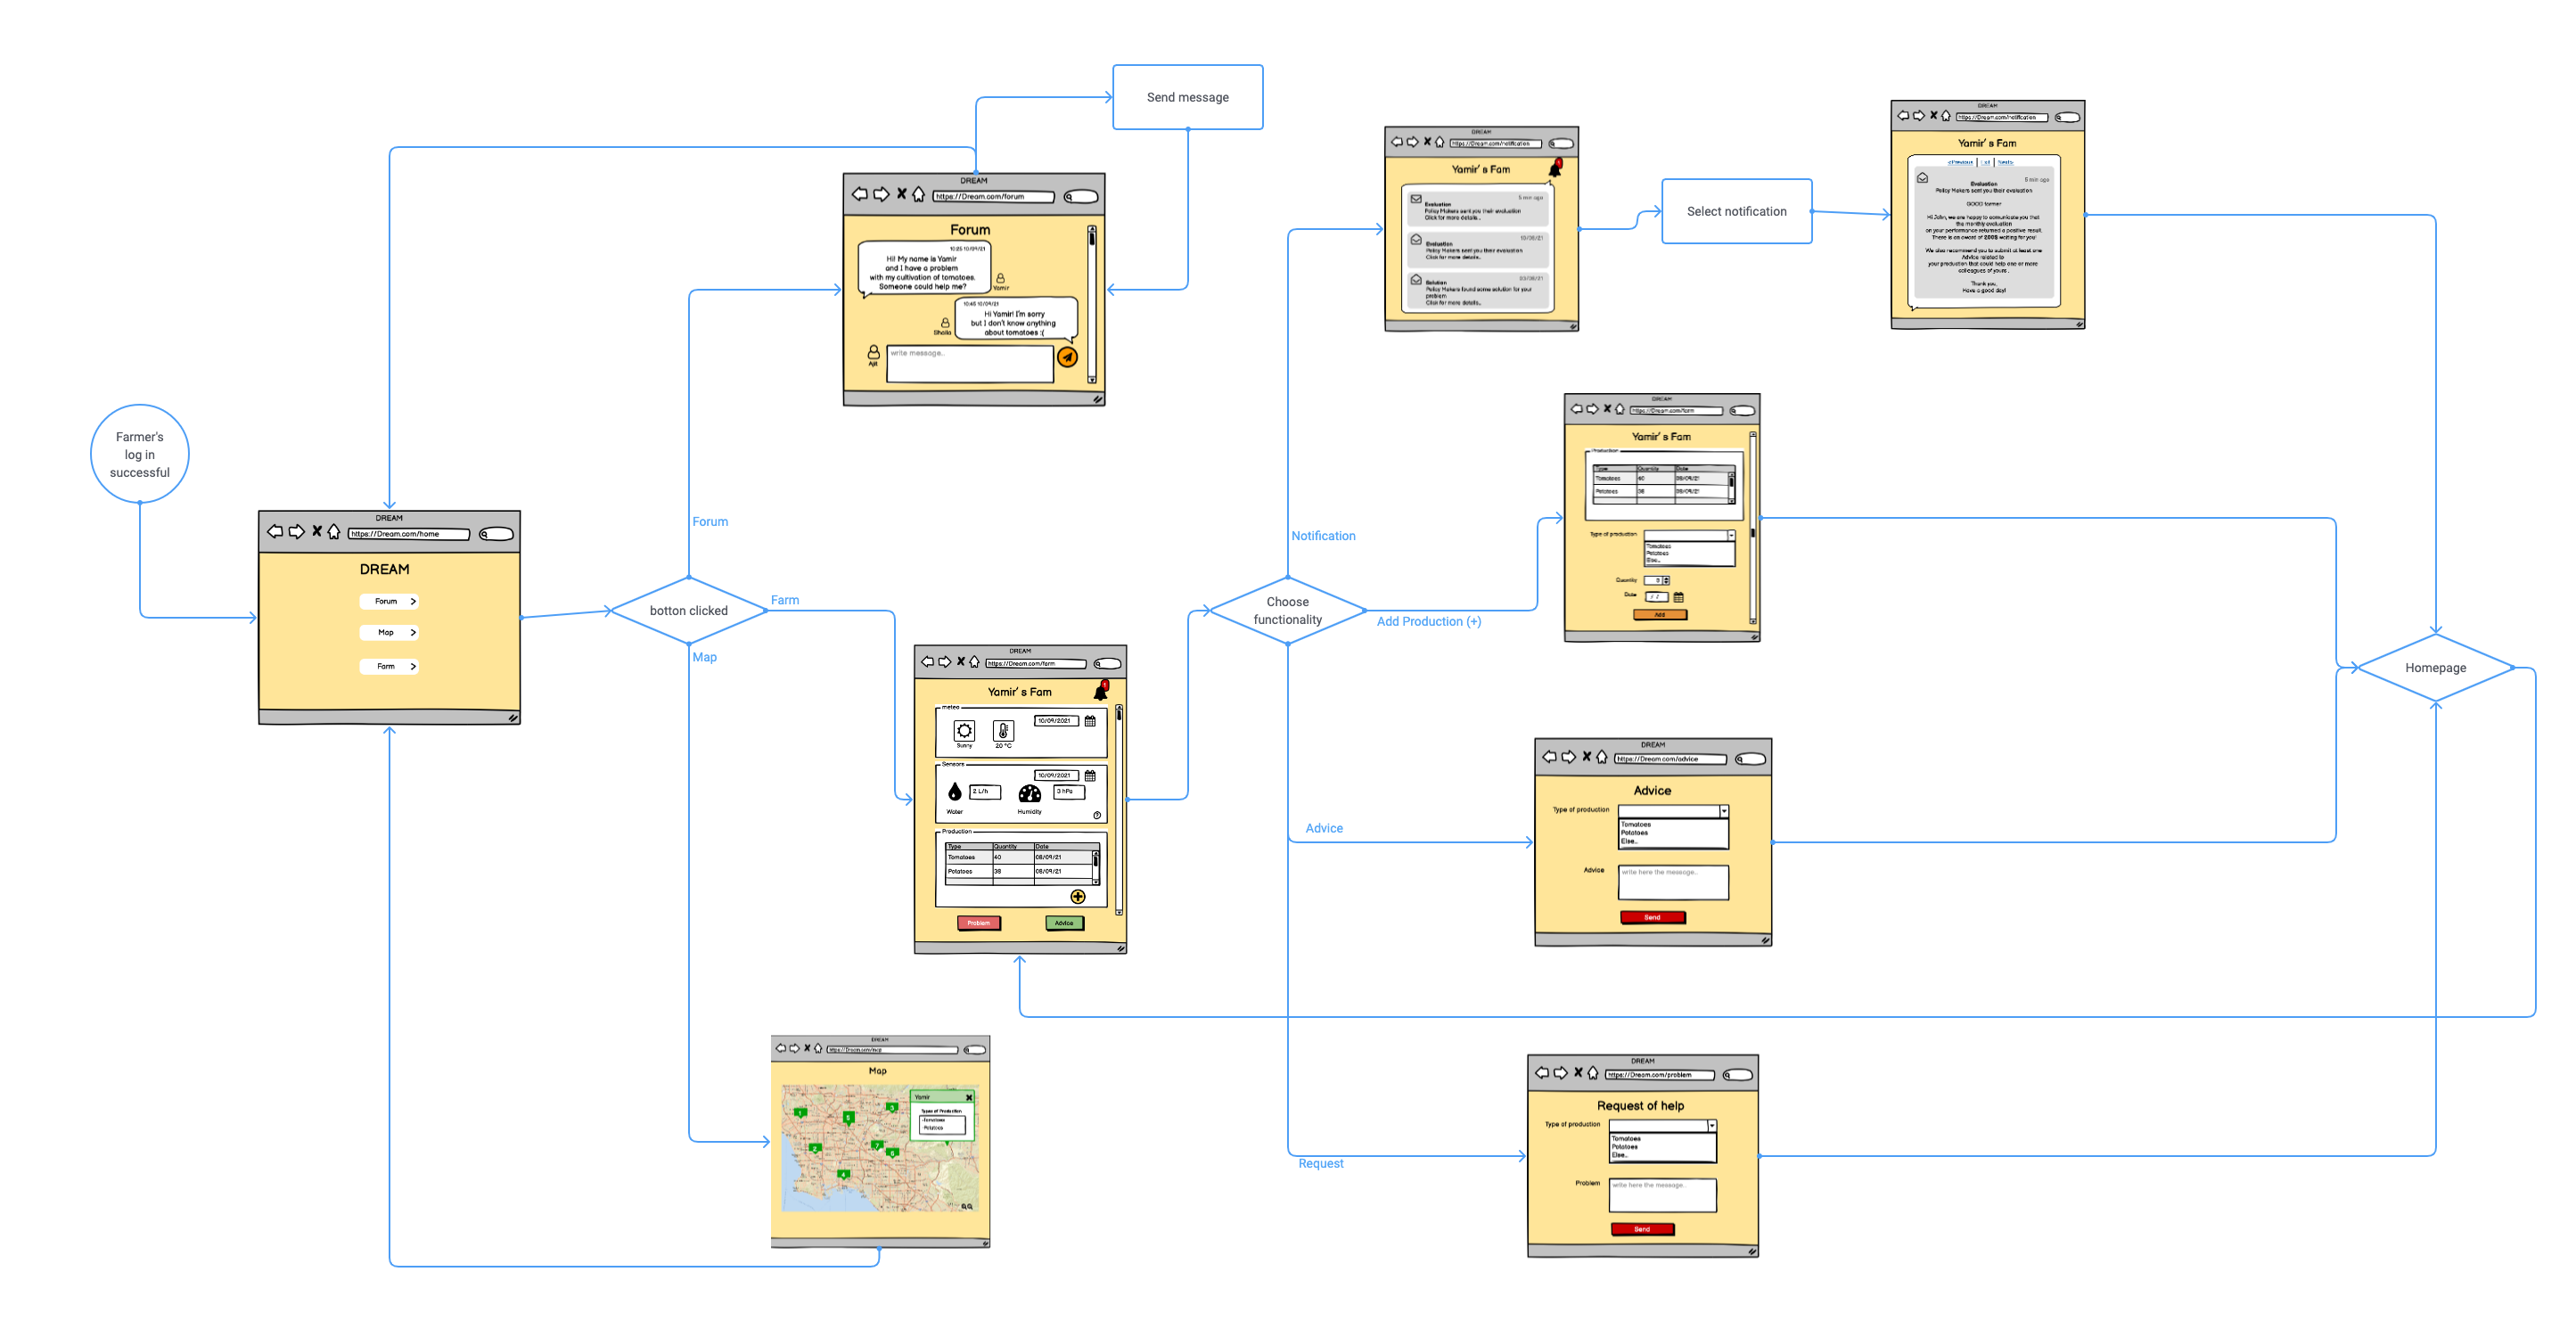
\includegraphics[width=1\textwidth]{images/UXdiagram_farmer.png}
          \caption{Farmer Web Application}
    \end{center}
\end{figure}
\begin{figure}[H]
    \begin{center}
          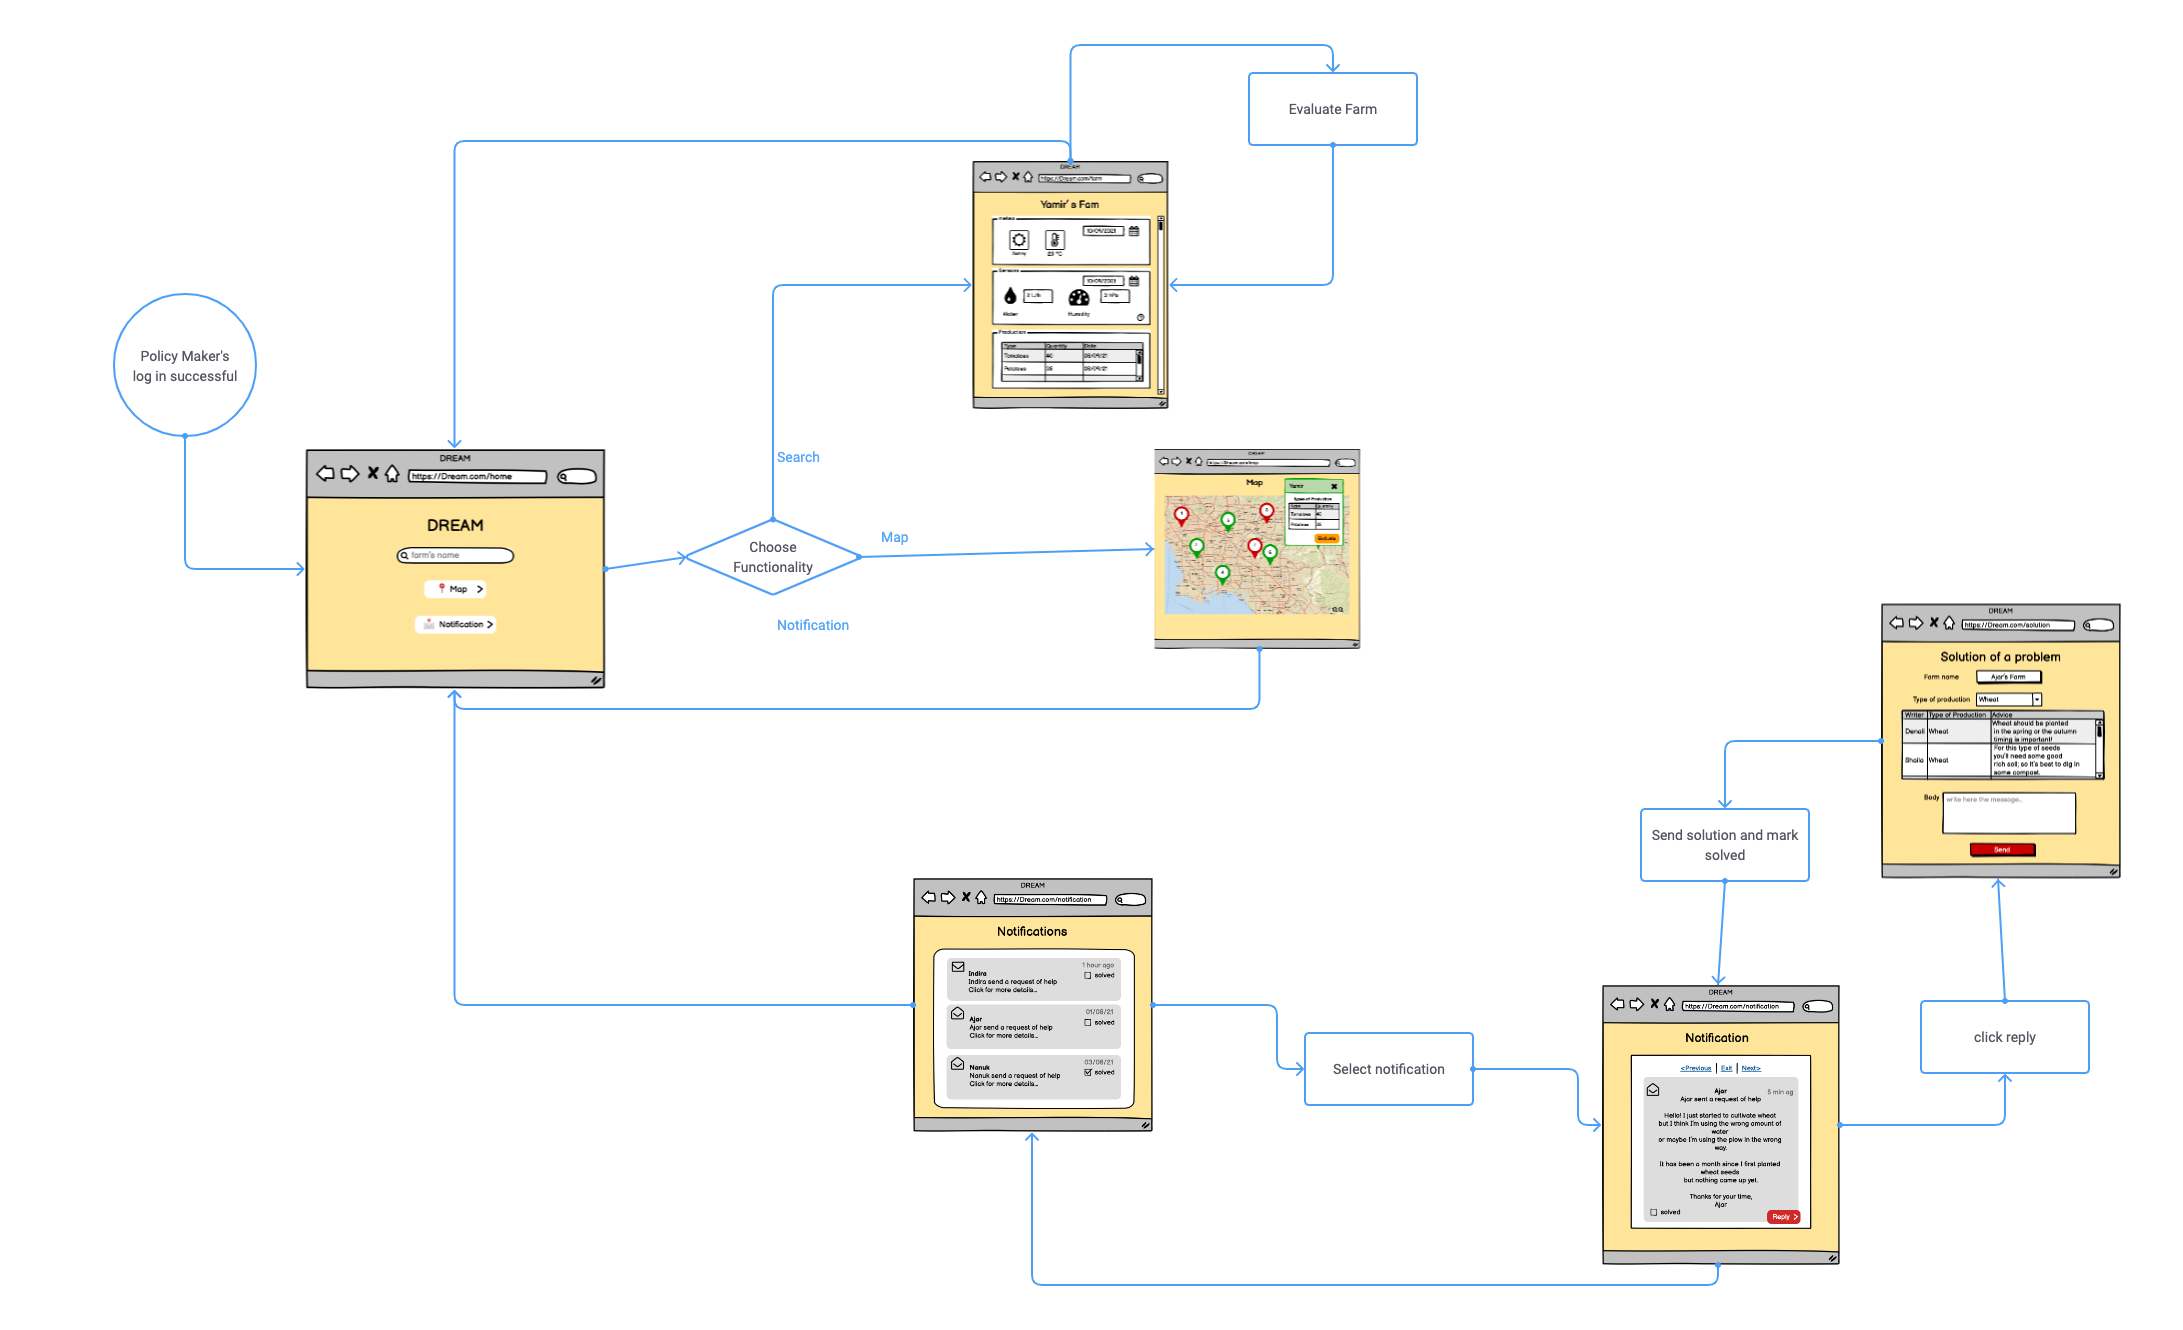
\includegraphics[width=1\textwidth]{images/UXdiagram_policymaker.png}
          \caption{Policy Maker Web Application}
    \end{center}
\end{figure}

\subsection{Web application}
\textbf{Dream's homepage} \\
The first mockup (Figure ..) is the first page that every user sees when accessing the web application. 
A user can click the button of the type of user that characterizes him.

\subsubsection{Farmer Web Application}
\textbf{Login}\\ 
The mockup showed in Figure .. is the initial page that every farmer sees after selecting the type of user. A farmer can interact with the application only 
after being authenticated. Therefore the farmer can decide to sign up if it is the first time ever that he uses the application or to login in through his authenticated credentials.
In order to login the user has to provide its email and his password. After being recognized he will be redirected to the home page which is going to be described in the next paragraphs.

\textbf{Registration} \\
The mockup showed in Figure .. is the sign up page, it allows the farmer to create a new account. This allows him to provide first the information related to his new account. 
Therefore he need to write his personal information: name, surname, email and password and in addition to that he must insert his farm name and position.
The sign up button will add the new farmer to the system and redirect the user to the login page where he can access the system.

\textbf{Homepage}\\
The homepage of the farmer's web application allows the user to select the features offered by the system:
\begin{itemize}
    \item Forum
    \item Map
    \item Farm
\end{itemize}
After clicking one of this buttons the farmer will be redirected to the selected pages, which are goin to be described in the next paragraphs.

\textbf{Forum}\\
The mockup in Figure .. shows a basic example of what the forum page will look like. The farmer on this page is able to read messages written by other farmer or 
write a message in order to answer or ask something to the other ones. After he types a message he need to click send in order to add the message in the application. 
After the button is clicked the user can see an updated version of this page.

\textbf{Map}\\
After selecting the map functionality on the homepage the user can see an updated version of the map, 
an example of it is showed in Figure ... The farmer on this page can see the location and name of the other farms and see what type of production 
they have.


\textbf{Farm Page}\\ 
The mockup showed in Figure .. is the homepage of the farm, the user can see here all the data that interest his farm. On top there is weather forecasting and data from sensor, r
egarding water consumption and humidity of soil. On the right corner there is a notification button, if it is clicked the system will redirect the user to the \textbf{notification page}(Figure ..).
Moreover on this page there are showed the most recent productions, divided by date and type. Clicking the '+' button the farmer can \textbf{insert new data}(Figure ...) that will be automatically be added to this list.
On the right bottom corner the user can click 'Problem' to \textbf{send a request} of help (Figure ..) or on the left 'Advice' to \textbf{send an advice} (Figure ..) that will be added to the system.


\subsubsection{Policy Maker Web Application}
\textbf{Login} \\
The mockup showed in Figure .. is the initial page that every policy maker sees after selecting the type of user.
A policy maker can interact with the system only after being authenticated. Therefore the policy maker needs to own the authentication code and password previously given to him.
Once being recognized the application will redirect him to the home page which is going to be described in the next paragraphs.

\textbf{Homepage} \\
After the successful login, the policy maker is redirected automatically to the homepage (Figure ..). 
In this page the application allows the user to select the features offered by the system:
\begin{itemize}
    \item Search
    \item Map
    \item Notifications
\end{itemize}
The first one permits the user to type the name of a farm in the search dialog in order to see all the information regarding that farm (Figure ..) and in addition he can review the evaluation if it is not done yet in that month.

\textbf{Map} \\
After selecting the map functionality on the homepage the user can see an updated version of the map, 
an example of it is showed in Figure ... 
The policy maker on this page can see the location and name of the farms in the area, see what type of production 
they have, their past evaluations and if in the last one they were evaluated positively or negatively.

\textbf{Notifications} \\
The notification page (Figure ..) shows all the requests sent by farmers. In order to read one of them the user must click on it. The notification now can be read (Figure ..) and can be solved or unsolved. 
If it is not solved yet the user can click on the reply button and answer it (Figure ..)


%-----------------------------------------------------------%
\newpage
\section{Requirements Traceability}
This section provides a mapping of the components descriped in section 2.2 with the requirements specified in the RASD.

\noindent\textbf{R1} The system must allow farmers to register\\
\indent \textbf{Access Manager, Registration Service}\\
\textbf{R2} The system must allow farmers to log in\\
\indent \textbf{Access Manager, Authentication Service}\\
\textbf{R3} The system must save the farmers registration data\\
\indent \textbf{Model, Data Manager}\\
\textbf{R4} The system must guarantee that each email address is unique\\
\indent \textbf{Registration Service}\\
\textbf{R5} The system must verify that the email address is valid\\
\indent \textbf{Registration Service}\\
\textbf{R6} The system must save the farmers information about their production submitted\\
\indent \textbf{Production Manager}\\
\textbf{R7} The system must allow farmers to insert the type of production \\
\indent \textbf{Production Manager}\\
\textbf{R8} The system must allow farmers to insert the amount of production type\\
\indent \textbf{Production Manager}\\
\textbf{R9} The system must allow farmers to specify a problem they faced to the Policy Makers\\
\indent \textbf{Notification Manager}\\
\textbf{R10} The system must allow farmers to select the type of production on which they had troubles\\
\indent \textbf{Notification Manager}\\
\textbf{R11} The system must save the advice submitted by the farmers\\
\indent \textbf{Notification Manager}\\
\textbf{R12} The system must allow farmers to select the type of product in their suggestion\\
\indent \textbf{Notification Manager}\\
\textbf{R13} The system must be able to show to the farmers advices send by the Policy Makers\\
\indent \textbf{Notification Manager}\\
\textbf{R14} The system must be able to show the meteorological data of the Farm’s position\\
\indent \textbf{View Info Manager, Weather Manager}\\
\textbf{R15} The system must be able to show the farm’s sensor data \\
\indent \textbf{View Info Manager, Data Manager, Model}\\
\textbf{R16} The system must allow farmers to send messages on the forum\\
\indent \textbf{Forum Manager}\\
\textbf{R17} The system must register date and time of a message in the forum\\
\indent \textbf{Forum Manager}\\
\textbf{R18} The system must be able to show all the messages on the forum\\
\indent \textbf{Forum Manager}\\
\textbf{R19} The system must be able to show the map of the zone\\
\indent \textbf{View Info Manager, Maps Manager}\\
\textbf{R20} The system must be able to show the farms position on the map\\
\indent \textbf{Maps Manager}\\
\textbf{R21} the system must be able to show on the map if a farm is performing well or not \\
\indent \textbf{Maps Manager}\\
\textbf{R22} The system must allow farmers to visualise notification send by Policy Makers\\
\indent \textbf{Notification Manager}\\
\textbf{R23} The system must allow farmers to see all information about his own farm\\
\indent \textbf{View Info Manager}\\
\textbf{R24} The system must be able to show the types of production cultivated in a farm\\
\indent \textbf{Maps Manager, Data Manager, Model}\\
\textbf{R25} The system must be able to show the quantity of product has been cultivated for each type in a farm\\
\indent \textbf{Production Manager}\\
\textbf{R26} The system does not allow Policy Makers to register\\
\indent \textbf{Access Manager}\\
\textbf{R27} The system must allow Policy Makers to log in\\
\indent \textbf{Authentication Service}\\
\textbf{R28} The system must verify that the code is valid\\
\indent \textbf{Authentication Service}\\
\textbf{R29} The system must allow Policy Makers to search a farm by name\\
\indent \textbf{Data Manager, Model}\\
\textbf{R30} The system must allow Policy Makers to see all farms’ pages\\
\indent \textbf{Data Manager, Model}\\
\textbf{R31} The system must not allow Policy Makers to modify any farm page\\
\indent \textbf{Authentication Service, Data Manager}\\
\textbf{R32} The system must allow Policy Makers to update the performance of a farmer\\
\indent \textbf{Notification Manager}\\
\textbf{R33} The system must allow Policy Makers to send notifications to the farmers\\
\indent \textbf{Notification Manager}\\
\textbf{R34} The system must allow Policy Makers to receive requests of help by the farmers\\
\indent \textbf{Notification Manager}\\

%-----------------------------------------------------------%
\newpage
\section{Implementation, Integration and Test Plan}
--Description--

External services do not need to be unit tested since it is assumed that they are reliable. 

[The order of the implementation, and why that one!]


\subsection{Plan Definition}
The strategy adopted for this phase of the project is a \textbf{bottom-up}: it focuses on individual components of the system. 
Starts from the detailed part, then links these ones to others and form larger components, until the entire system is formed. In this way it is possible to make decisions about low-level utilities and then decide how there will be put together to create high-level construct.\\ \\
In some cases we follow a \textbf{top-down} approach: start from an overview without going into details; then go deeper into more details each step. Top-down approach is used when a component needs another one that manages data it needs, but the second one is not implemented yet. In this way can be created hypothetical data while developing the main functionality. As a result we need to be able to generate feasible \textbf{stubs} used to simulate the data that the system is going to manage both real or randomly, in order to cover more scenarios possibles.\\ \\
The description starts from server's component because it is the most complex part and the core one that organize the hole system.\\
During the implementation \textbf{drivers} are used to simulate components that are not implemented yet, or to generate possible request.\\
The components that retreive information from external system are implemented later because they had no particular "intelligence" in it, are used only to retreive information and do not need big test on them(here are created the stub, their data are not relly crucial for the current step of the implementation) 

\begin{enumerate}
    \item This is the first step of the implementation. \\Most of the component require the performance of the \textsl{Model} and \textsl{Data Manager} to retrieve information and use hem to reply a user’s request. For this reason they are going to be implemented and tested first. 
    \begin{figure}[H]
        \begin{center}
        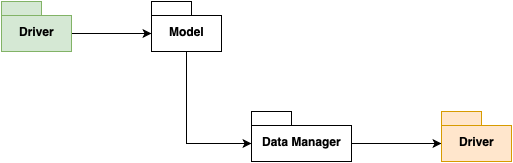
\includegraphics[width=1\textwidth]{implementation/step1.png}
        \caption{Implementation first step.}
        \label{fig:first step}
        \end{center}
    \end{figure}
    \item Then we start from the component that manage the access to the system. The reson is that this is a cructial phase of the application; it is how the user first approach the system and it's important that credential are well verified. The system must recognize the type of user to organize the application in the right way and reply with only the functionality permitted, so them affect the others components.\\ It is also a matter of privacy. 
    \begin{figure}[H]
        \begin{center}
        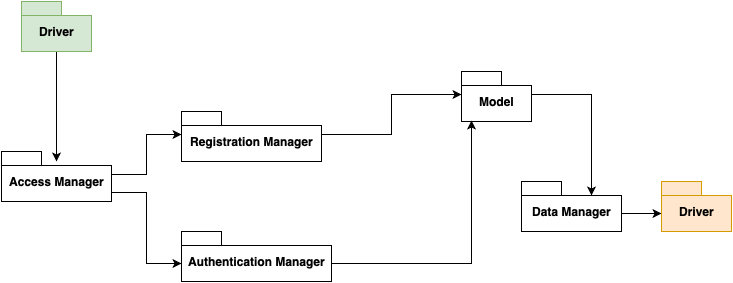
\includegraphics[width=1\textwidth]{implementation/step2.png}
        \caption{Implementation second step.}
        \label{fig:second step}
        \end{center}
    \end{figure}
    \item The main focus of the application is to help farmer with their production, so after the authentication the focus is on create the farm page with all the information that it requires. At first \textsl{Production Manager} to store or made visible the data about production and then \textsl{ViewInfo Manager} to create a first prototype of the farm page. Stub is used to fill the field in the page related to the weather.
    \begin{figure}[H]
        \begin{center}
        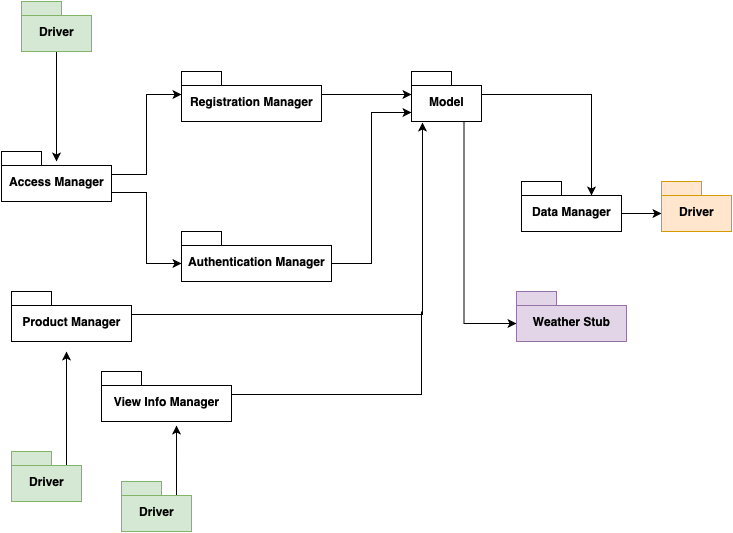
\includegraphics[width=1\textwidth]{implementation/step3.png}
        \caption{Implementation third step.}
        \label{fig:third step}
        \end{center}
    \end{figure}
    \item In this step the components related to the user ( \textsl{Web Servers} and \textsl{Web Application}) to create a real visualization and comuunication with these two part of the entire system, now that the main functionality can be used. A driver is used to create some possible request of the user and test the component yust integrated.
    \begin{figure}[H]
        \begin{center}
        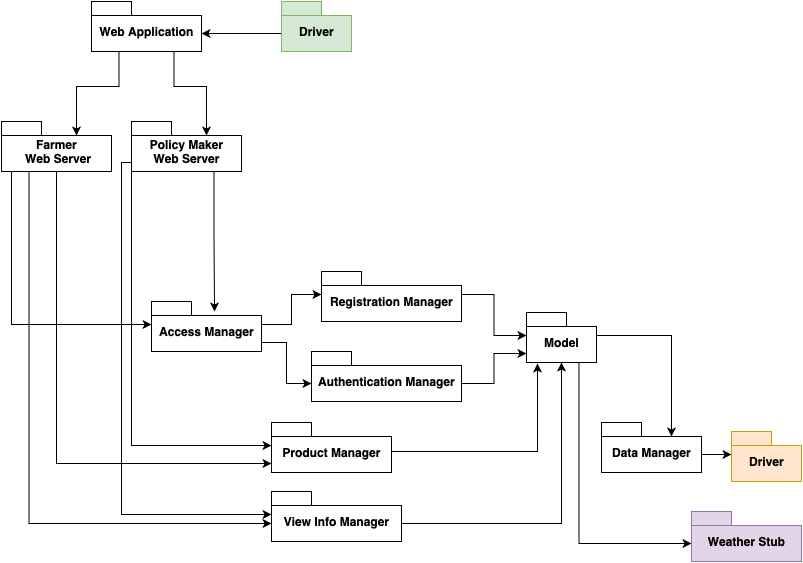
\includegraphics[width=1\textwidth]{implementation/step4.png}
        \caption{Implementation fourth step.}
        \label{fig:fourth step}
        \end{center}
    \end{figure}
    \item Now are added the components related to the other functionalities: retreive and send notification, with \textsl{Notification Manager} because farmer and policy maker ware "implemented" before, so it is possible to them to kind of comunicate through this component. The second functionality is to make able the farmers to comunicate to each other via forum, so the \textsl{Forum Manager} is created. The third is the visualization of the map so is integrated a stub just to test ifthge other components fill it with the right data. At this point all the pages can be created.
    \begin{figure}[H]
        \begin{center}
        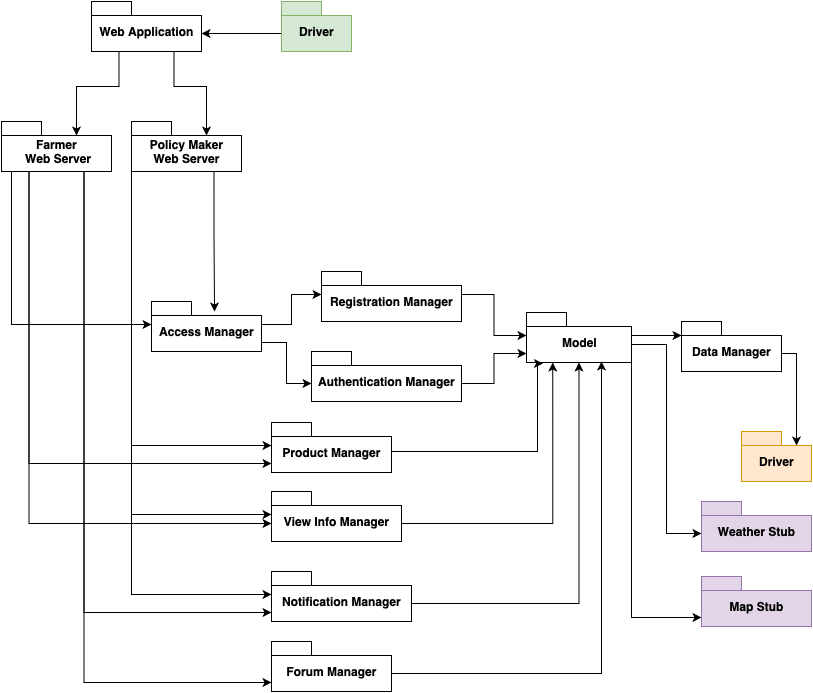
\includegraphics[width=1\textwidth]{implementation/step5.png}
        \caption{Implementation fifth step.}
        \label{fig:fifth step}
        \end{center}
    \end{figure}
    \item At least we integrate the components that comunicate with the external systems and retreive the real data, in the pages now are all "real" information. Now it is the implementation of the hole system.
    \begin{figure}[H]
        \begin{center}
        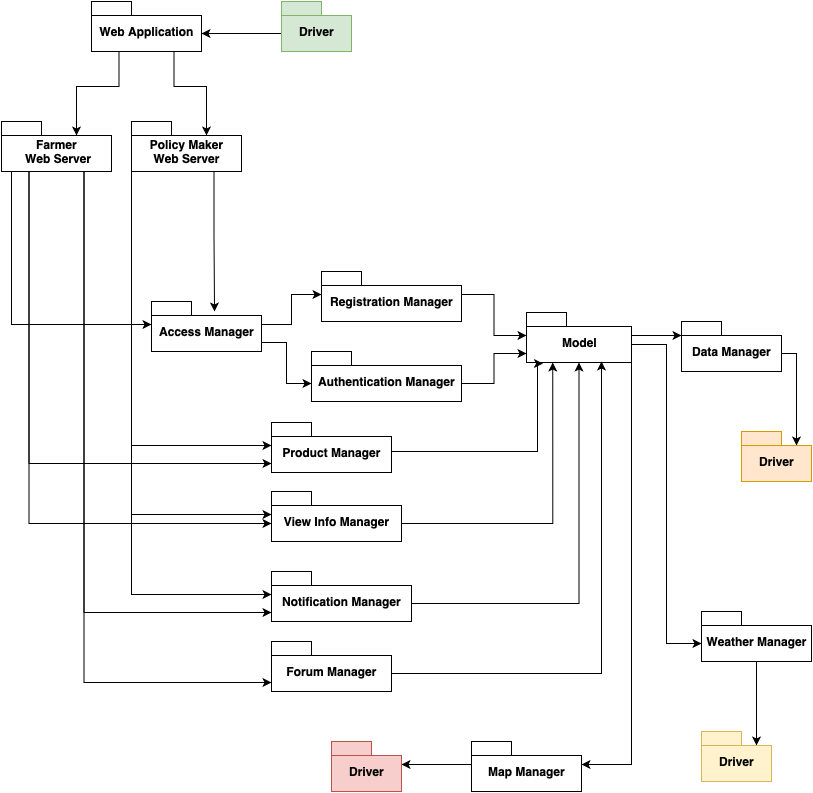
\includegraphics[width=1\textwidth]{implementation/step6.png}
        \caption{Implementation sixth step.}
        \label{fig:sixth step}
        \end{center}
    \end{figure}
\end{enumerate}



%-----------------------------------------------------------%
\newpage 
\section{Effort Spent}
\begin{table}[h]
      \centering
      \begin{tabular}{|p{3cm}||p{2cm}|p{2cm}|p{2cm}|p{2cm}|p{1cm}|}
            \hline
            Student & Time for S.1 & Time for S2 & Time for S.3 & Time for S.4 & Time for S.5\\
            \hline
            Valeria Detomas & h & h & h & h & h\\
            \hline
            Sofia Martellozzo & h & h & h & h & h\\
            \hline
      \end{tabular}
\end{table}

%-----------------------------------------------------------%
\section{Software and Tools used}
\begin{itemize}
      \item \LaTeX{} as document preparation system
      \item \href{https://lucid.co/}{Lucid}for the state chart 
      \item \href{https://sequencediagram.org}{SequenceDiagram.org} for the sequence diagrams
      \item \href{http://www.umletino.com/umletino.html}{Umletino} for UML diagram 
      \item \href{https://app.diagrams.net/}{Diagrams} for the use case diagram 
      \item \href{https://balsamiq.com}{Balsamig} for the mockups 
      \item \textbf{Alloy} as a model analyzer
      \item \href{https://github.com/}{GitHub} as verion control system.
\end{itemize}


%-----------------------------------------------------------%
\section{References}
\begin{itemize}
      \item Specification document: R\&DD Assignment A.Y. 2021-2022
      \item alloytool.org : Alloy Documentation
\end{itemize}

\end{document}
